\documentclass[twoside]{book}

% Packages required by doxygen
\usepackage{fixltx2e}
\usepackage{calc}
\usepackage{doxygen}
\usepackage[export]{adjustbox} % also loads graphicx
\usepackage{graphicx}
\usepackage[utf8]{inputenc}
\usepackage{makeidx}
\usepackage{multicol}
\usepackage{multirow}
\PassOptionsToPackage{warn}{textcomp}
\usepackage{textcomp}
\usepackage[nointegrals]{wasysym}
\usepackage[table]{xcolor}

% Font selection
\usepackage[T1]{fontenc}
\usepackage[scaled=.90]{helvet}
\usepackage{courier}
\usepackage{amssymb}
\usepackage{sectsty}
\renewcommand{\familydefault}{\sfdefault}
\allsectionsfont{%
  \fontseries{bc}\selectfont%
  \color{darkgray}%
}
\renewcommand{\DoxyLabelFont}{%
  \fontseries{bc}\selectfont%
  \color{darkgray}%
}
\newcommand{\+}{\discretionary{\mbox{\scriptsize$\hookleftarrow$}}{}{}}

% Page & text layout
\usepackage{geometry}
\geometry{%
  a4paper,%
  top=2.5cm,%
  bottom=2.5cm,%
  left=2.5cm,%
  right=2.5cm%
}
\tolerance=750
\hfuzz=15pt
\hbadness=750
\setlength{\emergencystretch}{15pt}
\setlength{\parindent}{0cm}
\setlength{\parskip}{3ex plus 2ex minus 2ex}
\makeatletter
\renewcommand{\paragraph}{%
  \@startsection{paragraph}{4}{0ex}{-1.0ex}{1.0ex}{%
    \normalfont\normalsize\bfseries\SS@parafont%
  }%
}
\renewcommand{\subparagraph}{%
  \@startsection{subparagraph}{5}{0ex}{-1.0ex}{1.0ex}{%
    \normalfont\normalsize\bfseries\SS@subparafont%
  }%
}
\makeatother

% Headers & footers
\usepackage{fancyhdr}
\pagestyle{fancyplain}
\fancyhead[LE]{\fancyplain{}{\bfseries\thepage}}
\fancyhead[CE]{\fancyplain{}{}}
\fancyhead[RE]{\fancyplain{}{\bfseries\leftmark}}
\fancyhead[LO]{\fancyplain{}{\bfseries\rightmark}}
\fancyhead[CO]{\fancyplain{}{}}
\fancyhead[RO]{\fancyplain{}{\bfseries\thepage}}
\fancyfoot[LE]{\fancyplain{}{}}
\fancyfoot[CE]{\fancyplain{}{}}
\fancyfoot[RE]{\fancyplain{}{\bfseries\scriptsize Generated by Doxygen }}
\fancyfoot[LO]{\fancyplain{}{\bfseries\scriptsize Generated by Doxygen }}
\fancyfoot[CO]{\fancyplain{}{}}
\fancyfoot[RO]{\fancyplain{}{}}
\renewcommand{\footrulewidth}{0.4pt}
\renewcommand{\chaptermark}[1]{%
  \markboth{#1}{}%
}
\renewcommand{\sectionmark}[1]{%
  \markright{\thesection\ #1}%
}

% Indices & bibliography
\usepackage{natbib}
\usepackage[titles]{tocloft}
\setcounter{tocdepth}{3}
\setcounter{secnumdepth}{5}
\makeindex

% Hyperlinks (required, but should be loaded last)
\usepackage{ifpdf}
\ifpdf
  \usepackage[pdftex,pagebackref=true]{hyperref}
\else
  \usepackage[ps2pdf,pagebackref=true]{hyperref}
\fi
\hypersetup{%
  colorlinks=true,%
  linkcolor=blue,%
  citecolor=blue,%
  unicode%
}

% Custom commands
\newcommand{\clearemptydoublepage}{%
  \newpage{\pagestyle{empty}\cleardoublepage}%
}

\usepackage{caption}
\captionsetup{labelsep=space,justification=centering,font={bf},singlelinecheck=off,skip=4pt,position=top}

%===== C O N T E N T S =====

\begin{document}

% Titlepage & ToC
\hypersetup{pageanchor=false,
             bookmarksnumbered=true,
             pdfencoding=unicode
            }
\pagenumbering{roman}
\begin{titlepage}
\vspace*{7cm}
\begin{center}%
{\Large My Project }\\
\vspace*{1cm}
{\large Generated by Doxygen 1.8.11}\\
\end{center}
\end{titlepage}
\clearemptydoublepage
\tableofcontents
\clearemptydoublepage
\pagenumbering{arabic}
\hypersetup{pageanchor=true}

%--- Begin generated contents ---
\chapter{Namespace Index}
\section{Namespace List}
Here is a list of all namespaces with brief descriptions\+:\begin{DoxyCompactList}
\item\contentsline{section}{\hyperlink{namespace_maike}{Maike} }{\pageref{namespace_maike}}{}
\end{DoxyCompactList}

\chapter{Hierarchical Index}
\section{Class Hierarchy}
This inheritance list is sorted roughly, but not completely, alphabetically\+:\begin{DoxyCompactList}
\item \contentsline{section}{Maike\+:\+:Dependency}{\pageref{class_maike_1_1_dependency}}{}
\item \contentsline{section}{Maike\+:\+:Dependency\+Graph}{\pageref{class_maike_1_1_dependency_graph}}{}
\begin{DoxyCompactList}
\item \contentsline{section}{Maike\+:\+:Dependency\+Graph\+Default}{\pageref{class_maike_1_1_dependency_graph_default}}{}
\end{DoxyCompactList}
\item \contentsline{section}{Maike\+:\+:Invoker}{\pageref{class_maike_1_1_invoker}}{}
\begin{DoxyCompactList}
\item \contentsline{section}{Maike\+:\+:Invoker\+Real}{\pageref{class_maike_1_1_invoker_real}}{}
\end{DoxyCompactList}
\item pair\begin{DoxyCompactList}
\item \contentsline{section}{Maike\+:\+:Twins$<$ T $>$}{\pageref{struct_maike_1_1_twins}}{}
\end{DoxyCompactList}
\item \contentsline{section}{Maike\+:\+:Spider}{\pageref{class_maike_1_1_spider}}{}
\item \contentsline{section}{Maike\+:\+:Target}{\pageref{class_maike_1_1_target}}{}
\item \contentsline{section}{Maike\+:\+:Target\+Loader}{\pageref{class_maike_1_1_target_loader}}{}
\item \contentsline{section}{Maike\+:\+:Dependency\+Graph\+:\+:Target\+Processor}{\pageref{class_maike_1_1_dependency_graph_1_1_target_processor}}{}
\begin{DoxyCompactList}
\item \contentsline{section}{Leaf\+Collector}{\pageref{class_leaf_collector}}{}
\end{DoxyCompactList}
\end{DoxyCompactList}

\chapter{Class Index}
\section{Class List}
Here are the classes, structs, unions and interfaces with brief descriptions\+:\begin{DoxyCompactList}
\item\contentsline{section}{\hyperlink{class_maike_1_1_dependency}{Maike\+::\+Dependency} }{\pageref{class_maike_1_1_dependency}}{}
\item\contentsline{section}{\hyperlink{class_maike_1_1_dependency_graph}{Maike\+::\+Dependency\+Graph} }{\pageref{class_maike_1_1_dependency_graph}}{}
\item\contentsline{section}{\hyperlink{class_maike_1_1_dependency_graph_default}{Maike\+::\+Dependency\+Graph\+Default} }{\pageref{class_maike_1_1_dependency_graph_default}}{}
\item\contentsline{section}{\hyperlink{class_maike_1_1_invoker}{Maike\+::\+Invoker} }{\pageref{class_maike_1_1_invoker}}{}
\item\contentsline{section}{\hyperlink{class_maike_1_1_invoker_real}{Maike\+::\+Invoker\+Real} }{\pageref{class_maike_1_1_invoker_real}}{}
\item\contentsline{section}{\hyperlink{class_leaf_collector}{Leaf\+Collector} }{\pageref{class_leaf_collector}}{}
\item\contentsline{section}{\hyperlink{class_maike_1_1_spider}{Maike\+::\+Spider} }{\pageref{class_maike_1_1_spider}}{}
\item\contentsline{section}{\hyperlink{class_maike_1_1_target}{Maike\+::\+Target} }{\pageref{class_maike_1_1_target}}{}
\item\contentsline{section}{\hyperlink{class_maike_1_1_target_loader}{Maike\+::\+Target\+Loader} }{\pageref{class_maike_1_1_target_loader}}{}
\item\contentsline{section}{\hyperlink{class_maike_1_1_dependency_graph_1_1_target_processor}{Maike\+::\+Dependency\+Graph\+::\+Target\+Processor} }{\pageref{class_maike_1_1_dependency_graph_1_1_target_processor}}{}
\item\contentsline{section}{\hyperlink{struct_maike_1_1_twins}{Maike\+::\+Twins$<$ T $>$} }{\pageref{struct_maike_1_1_twins}}{}
\end{DoxyCompactList}

\chapter{File Index}
\section{File List}
Here is a list of all files with brief descriptions\+:\begin{DoxyCompactList}
\item\contentsline{section}{\hyperlink{dependency_8cpp}{dependency.\+cpp} }{\pageref{dependency_8cpp}}{}
\item\contentsline{section}{\hyperlink{dependency_8hpp}{dependency.\+hpp} }{\pageref{dependency_8hpp}}{}
\item\contentsline{section}{\hyperlink{dependencygraph_8hpp}{dependencygraph.\+hpp} }{\pageref{dependencygraph_8hpp}}{}
\item\contentsline{section}{\hyperlink{dependencygraphdefault_8cpp}{dependencygraphdefault.\+cpp} }{\pageref{dependencygraphdefault_8cpp}}{}
\item\contentsline{section}{\hyperlink{dependencygraphdefault_8hpp}{dependencygraphdefault.\+hpp} }{\pageref{dependencygraphdefault_8hpp}}{}
\item\contentsline{section}{\hyperlink{invoker_8hpp}{invoker.\+hpp} }{\pageref{invoker_8hpp}}{}
\item\contentsline{section}{\hyperlink{invokerreal_8hpp}{invokerreal.\+hpp} }{\pageref{invokerreal_8hpp}}{}
\item\contentsline{section}{\hyperlink{maike-main_8cpp}{maike-\/main.\+cpp} }{\pageref{maike-main_8cpp}}{}
\item\contentsline{section}{\hyperlink{maike_8cpp}{maike.\+cpp} }{\pageref{maike_8cpp}}{}
\item\contentsline{section}{\hyperlink{maike_8hpp}{maike.\+hpp} }{\pageref{maike_8hpp}}{}
\item\contentsline{section}{\hyperlink{spider_8hpp}{spider.\+hpp} }{\pageref{spider_8hpp}}{}
\item\contentsline{section}{\hyperlink{target_8cpp}{target.\+cpp} }{\pageref{target_8cpp}}{}
\item\contentsline{section}{\hyperlink{target_8hpp}{target.\+hpp} }{\pageref{target_8hpp}}{}
\item\contentsline{section}{\hyperlink{targetloader_8hpp}{targetloader.\+hpp} }{\pageref{targetloader_8hpp}}{}
\item\contentsline{section}{\hyperlink{twins_8hpp}{twins.\+hpp} }{\pageref{twins_8hpp}}{}
\end{DoxyCompactList}

\chapter{Namespace Documentation}
\hypertarget{namespace_maike}{}\section{Maike Namespace Reference}
\label{namespace_maike}\index{Maike@{Maike}}
\subsection*{Classes}
\begin{DoxyCompactItemize}
\item 
class \hyperlink{class_maike_1_1_dependency}{Dependency}
\item 
class \hyperlink{class_maike_1_1_dependency_graph}{Dependency\+Graph}
\item 
class \hyperlink{class_maike_1_1_dependency_graph_default}{Dependency\+Graph\+Default}
\item 
class \hyperlink{class_maike_1_1_invoker}{Invoker}
\item 
class \hyperlink{class_maike_1_1_invoker_real}{Invoker\+Real}
\item 
class \hyperlink{class_maike_1_1_spider}{Spider}
\item 
class \hyperlink{class_maike_1_1_target}{Target}
\item 
class \hyperlink{class_maike_1_1_target_loader}{Target\+Loader}
\item 
struct \hyperlink{struct_maike_1_1_twins}{Twins}
\end{DoxyCompactItemize}
\subsection*{Functions}
\begin{DoxyCompactItemize}
\item 
void \hyperlink{namespace_maike_a1b65c50ccc0ce45272d1eb6557057ec0}{build\+Branch} (\hyperlink{class_maike_1_1_target}{Target} \&target, \hyperlink{class_maike_1_1_invoker}{Invoker} \&invoker, size\+\_\+t targets\+\_\+count)
\item 
void \hyperlink{namespace_maike_aed76b0165d074646da9cfa1ad7bfc5b7}{build\+All} (\hyperlink{struct_maike_1_1_twins}{Twins}$<$ \hyperlink{class_maike_1_1_target}{Target} $\ast$ $>$ leafs, \hyperlink{class_maike_1_1_invoker}{Invoker} \&invoker, size\+\_\+t targets\+\_\+count)
\end{DoxyCompactItemize}


\subsection{Function Documentation}
\index{Maike@{Maike}!build\+All@{build\+All}}
\index{build\+All@{build\+All}!Maike@{Maike}}
\subsubsection[{\texorpdfstring{build\+All(\+Twins$<$ Target $\ast$ $>$ leafs, Invoker \&invoker, size\+\_\+t targets\+\_\+count)}{buildAll(Twins< Target * > leafs, Invoker &invoker, size_t targets_count)}}]{\setlength{\rightskip}{0pt plus 5cm}void Maike\+::build\+All (
\begin{DoxyParamCaption}
\item[{{\bf Twins}$<$ {\bf Target} $\ast$ $>$}]{leafs, }
\item[{{\bf Invoker} \&}]{invoker, }
\item[{size\+\_\+t}]{targets\+\_\+count}
\end{DoxyParamCaption}
)}\hypertarget{namespace_maike_aed76b0165d074646da9cfa1ad7bfc5b7}{}\label{namespace_maike_aed76b0165d074646da9cfa1ad7bfc5b7}
\index{Maike@{Maike}!build\+Branch@{build\+Branch}}
\index{build\+Branch@{build\+Branch}!Maike@{Maike}}
\subsubsection[{\texorpdfstring{build\+Branch(\+Target \&target, Invoker \&invoker, size\+\_\+t targets\+\_\+count)}{buildBranch(Target &target, Invoker &invoker, size_t targets_count)}}]{\setlength{\rightskip}{0pt plus 5cm}void Maike\+::build\+Branch (
\begin{DoxyParamCaption}
\item[{{\bf Target} \&}]{target, }
\item[{{\bf Invoker} \&}]{invoker, }
\item[{size\+\_\+t}]{targets\+\_\+count}
\end{DoxyParamCaption}
)}\hypertarget{namespace_maike_a1b65c50ccc0ce45272d1eb6557057ec0}{}\label{namespace_maike_a1b65c50ccc0ce45272d1eb6557057ec0}

\chapter{Class Documentation}
\hypertarget{class_maike_1_1_dependency}{}\section{Maike\+:\+:Dependency Class Reference}
\label{class_maike_1_1_dependency}\index{Maike\+::\+Dependency@{Maike\+::\+Dependency}}


{\ttfamily \#include $<$dependency.\+hpp$>$}



Collaboration diagram for Maike\+:\+:Dependency\+:\nopagebreak
\begin{figure}[H]
\begin{center}
\leavevmode
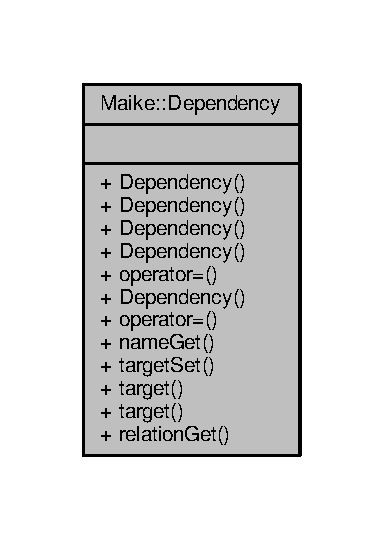
\includegraphics[width=184pt]{class_maike_1_1_dependency__coll__graph}
\end{center}
\end{figure}
\subsection*{Public Types}
\begin{DoxyCompactItemize}
\item 
enum \hyperlink{class_maike_1_1_dependency_a1b670303409ad2240f246e2a2c55d380}{Relation} \+: unsigned int \{ \hyperlink{class_maike_1_1_dependency_a1b670303409ad2240f246e2a2c55d380a5c19bc679506425e481a34caff777350}{Relation\+::\+L\+E\+AF}, 
\hyperlink{class_maike_1_1_dependency_a1b670303409ad2240f246e2a2c55d380a182fa1c42a2468f8488e6dcf75a81b81}{Relation\+::\+I\+N\+T\+E\+R\+N\+AL}, 
\hyperlink{class_maike_1_1_dependency_a1b670303409ad2240f246e2a2c55d380a8721d9c72777f66c96863a998e48adc3}{Relation\+::\+I\+M\+P\+L\+E\+M\+E\+N\+T\+A\+T\+I\+ON}, 
\hyperlink{class_maike_1_1_dependency_a1b670303409ad2240f246e2a2c55d380a3932d629fb5e2be9d09b3a4485b3cc9d}{Relation\+::\+E\+X\+T\+E\+R\+N\+AL}
 \}
\end{DoxyCompactItemize}
\subsection*{Public Member Functions}
\begin{DoxyCompactItemize}
\item 
\hyperlink{class_maike_1_1_dependency_aa92957076c5000d1d3a56073302f1a41}{Dependency} ()
\item 
\hyperlink{class_maike_1_1_dependency_aaec77bca6441a19bd17a5d4c598597c3}{Dependency} (\hyperlink{class_maike_1_1_target}{Target} \&\hyperlink{class_maike_1_1_dependency_a80ef5cd5a250b6bcbf8425bedf7c4498}{target})
\item 
\hyperlink{class_maike_1_1_dependency_aad801e78c273acc7d8d228eb4ad27c56}{Dependency} (const char $\ast$name, \hyperlink{class_maike_1_1_dependency_a1b670303409ad2240f246e2a2c55d380}{Relation} relation)
\item 
\hyperlink{class_maike_1_1_dependency_ae8f606939c5f403c450ac453fdcd231a}{Dependency} (const \hyperlink{class_maike_1_1_dependency}{Dependency} \&)=default
\item 
\hyperlink{class_maike_1_1_dependency}{Dependency} \& \hyperlink{class_maike_1_1_dependency_ab14650c3df3a66c1003966e64ac7ad3d}{operator=} (const \hyperlink{class_maike_1_1_dependency}{Dependency} \&)=default
\item 
\hyperlink{class_maike_1_1_dependency_a8385a5d634240be722dca5ebf908c0c5}{Dependency} (\hyperlink{class_maike_1_1_dependency}{Dependency} \&\&)=default
\item 
\hyperlink{class_maike_1_1_dependency}{Dependency} \& \hyperlink{class_maike_1_1_dependency_a00da6c0f5d5b654a8d4412b90034655f}{operator=} (\hyperlink{class_maike_1_1_dependency}{Dependency} \&\&)=default
\item 
const char $\ast$ \hyperlink{class_maike_1_1_dependency_aa24f1895d1a46b19c33847f10d6cce12}{name\+Get} () const noexcept
\item 
\hyperlink{class_maike_1_1_dependency}{Dependency} \& \hyperlink{class_maike_1_1_dependency_a787830159fe8c1886e7d37881c26a905}{target\+Set} (\hyperlink{class_maike_1_1_target}{Target} \&\hyperlink{class_maike_1_1_dependency_a80ef5cd5a250b6bcbf8425bedf7c4498}{target}) noexcept
\item 
\hyperlink{class_maike_1_1_target}{Target} $\ast$ \hyperlink{class_maike_1_1_dependency_a80ef5cd5a250b6bcbf8425bedf7c4498}{target} () noexcept
\item 
const \hyperlink{class_maike_1_1_target}{Target} $\ast$ \hyperlink{class_maike_1_1_dependency_a702f6a338fdf2712b5fe697bb16b10fb}{target} () const noexcept
\item 
\hyperlink{class_maike_1_1_dependency_a1b670303409ad2240f246e2a2c55d380}{Relation} \hyperlink{class_maike_1_1_dependency_ad92e460b2e708a9ea0014cf80e0f80a1}{relation\+Get} () const noexcept
\end{DoxyCompactItemize}


\subsection{Member Enumeration Documentation}
\index{Maike\+::\+Dependency@{Maike\+::\+Dependency}!Relation@{Relation}}
\index{Relation@{Relation}!Maike\+::\+Dependency@{Maike\+::\+Dependency}}
\subsubsection[{\texorpdfstring{Relation}{Relation}}]{\setlength{\rightskip}{0pt plus 5cm}enum {\bf Maike\+::\+Dependency\+::\+Relation} \+: unsigned int\hspace{0.3cm}{\ttfamily [strong]}}\hypertarget{class_maike_1_1_dependency_a1b670303409ad2240f246e2a2c55d380}{}\label{class_maike_1_1_dependency_a1b670303409ad2240f246e2a2c55d380}
\begin{Desc}
\item[Enumerator]\par
\begin{description}
\index{L\+E\+AF@{L\+E\+AF}!Maike\+::\+Dependency@{Maike\+::\+Dependency}}\index{Maike\+::\+Dependency@{Maike\+::\+Dependency}!L\+E\+AF@{L\+E\+AF}}\item[{\em 
L\+E\+AF\hypertarget{class_maike_1_1_dependency_a1b670303409ad2240f246e2a2c55d380a5c19bc679506425e481a34caff777350}{}\label{class_maike_1_1_dependency_a1b670303409ad2240f246e2a2c55d380a5c19bc679506425e481a34caff777350}
}]\index{I\+N\+T\+E\+R\+N\+AL@{I\+N\+T\+E\+R\+N\+AL}!Maike\+::\+Dependency@{Maike\+::\+Dependency}}\index{Maike\+::\+Dependency@{Maike\+::\+Dependency}!I\+N\+T\+E\+R\+N\+AL@{I\+N\+T\+E\+R\+N\+AL}}\item[{\em 
I\+N\+T\+E\+R\+N\+AL\hypertarget{class_maike_1_1_dependency_a1b670303409ad2240f246e2a2c55d380a182fa1c42a2468f8488e6dcf75a81b81}{}\label{class_maike_1_1_dependency_a1b670303409ad2240f246e2a2c55d380a182fa1c42a2468f8488e6dcf75a81b81}
}]\index{I\+M\+P\+L\+E\+M\+E\+N\+T\+A\+T\+I\+ON@{I\+M\+P\+L\+E\+M\+E\+N\+T\+A\+T\+I\+ON}!Maike\+::\+Dependency@{Maike\+::\+Dependency}}\index{Maike\+::\+Dependency@{Maike\+::\+Dependency}!I\+M\+P\+L\+E\+M\+E\+N\+T\+A\+T\+I\+ON@{I\+M\+P\+L\+E\+M\+E\+N\+T\+A\+T\+I\+ON}}\item[{\em 
I\+M\+P\+L\+E\+M\+E\+N\+T\+A\+T\+I\+ON\hypertarget{class_maike_1_1_dependency_a1b670303409ad2240f246e2a2c55d380a8721d9c72777f66c96863a998e48adc3}{}\label{class_maike_1_1_dependency_a1b670303409ad2240f246e2a2c55d380a8721d9c72777f66c96863a998e48adc3}
}]\index{E\+X\+T\+E\+R\+N\+AL@{E\+X\+T\+E\+R\+N\+AL}!Maike\+::\+Dependency@{Maike\+::\+Dependency}}\index{Maike\+::\+Dependency@{Maike\+::\+Dependency}!E\+X\+T\+E\+R\+N\+AL@{E\+X\+T\+E\+R\+N\+AL}}\item[{\em 
E\+X\+T\+E\+R\+N\+AL\hypertarget{class_maike_1_1_dependency_a1b670303409ad2240f246e2a2c55d380a3932d629fb5e2be9d09b3a4485b3cc9d}{}\label{class_maike_1_1_dependency_a1b670303409ad2240f246e2a2c55d380a3932d629fb5e2be9d09b3a4485b3cc9d}
}]\end{description}
\end{Desc}


\subsection{Constructor \& Destructor Documentation}
\index{Maike\+::\+Dependency@{Maike\+::\+Dependency}!Dependency@{Dependency}}
\index{Dependency@{Dependency}!Maike\+::\+Dependency@{Maike\+::\+Dependency}}
\subsubsection[{\texorpdfstring{Dependency()}{Dependency()}}]{\setlength{\rightskip}{0pt plus 5cm}Dependency\+::\+Dependency (
\begin{DoxyParamCaption}
{}
\end{DoxyParamCaption}
)}\hypertarget{class_maike_1_1_dependency_aa92957076c5000d1d3a56073302f1a41}{}\label{class_maike_1_1_dependency_aa92957076c5000d1d3a56073302f1a41}
\index{Maike\+::\+Dependency@{Maike\+::\+Dependency}!Dependency@{Dependency}}
\index{Dependency@{Dependency}!Maike\+::\+Dependency@{Maike\+::\+Dependency}}
\subsubsection[{\texorpdfstring{Dependency(\+Target \&target)}{Dependency(Target &target)}}]{\setlength{\rightskip}{0pt plus 5cm}Maike\+::\+Dependency\+::\+Dependency (
\begin{DoxyParamCaption}
\item[{{\bf Target} \&}]{target}
\end{DoxyParamCaption}
)\hspace{0.3cm}{\ttfamily [inline]}, {\ttfamily [explicit]}}\hypertarget{class_maike_1_1_dependency_aaec77bca6441a19bd17a5d4c598597c3}{}\label{class_maike_1_1_dependency_aaec77bca6441a19bd17a5d4c598597c3}
\index{Maike\+::\+Dependency@{Maike\+::\+Dependency}!Dependency@{Dependency}}
\index{Dependency@{Dependency}!Maike\+::\+Dependency@{Maike\+::\+Dependency}}
\subsubsection[{\texorpdfstring{Dependency(const char $\ast$name, Relation relation)}{Dependency(const char *name, Relation relation)}}]{\setlength{\rightskip}{0pt plus 5cm}Dependency\+::\+Dependency (
\begin{DoxyParamCaption}
\item[{const char $\ast$}]{name, }
\item[{{\bf Relation}}]{relation}
\end{DoxyParamCaption}
)\hspace{0.3cm}{\ttfamily [explicit]}}\hypertarget{class_maike_1_1_dependency_aad801e78c273acc7d8d228eb4ad27c56}{}\label{class_maike_1_1_dependency_aad801e78c273acc7d8d228eb4ad27c56}
\index{Maike\+::\+Dependency@{Maike\+::\+Dependency}!Dependency@{Dependency}}
\index{Dependency@{Dependency}!Maike\+::\+Dependency@{Maike\+::\+Dependency}}
\subsubsection[{\texorpdfstring{Dependency(const Dependency \&)=default}{Dependency(const Dependency &)=default}}]{\setlength{\rightskip}{0pt plus 5cm}Maike\+::\+Dependency\+::\+Dependency (
\begin{DoxyParamCaption}
\item[{const {\bf Dependency} \&}]{}
\end{DoxyParamCaption}
)\hspace{0.3cm}{\ttfamily [default]}}\hypertarget{class_maike_1_1_dependency_ae8f606939c5f403c450ac453fdcd231a}{}\label{class_maike_1_1_dependency_ae8f606939c5f403c450ac453fdcd231a}
\index{Maike\+::\+Dependency@{Maike\+::\+Dependency}!Dependency@{Dependency}}
\index{Dependency@{Dependency}!Maike\+::\+Dependency@{Maike\+::\+Dependency}}
\subsubsection[{\texorpdfstring{Dependency(\+Dependency \&\&)=default}{Dependency(Dependency &&)=default}}]{\setlength{\rightskip}{0pt plus 5cm}Maike\+::\+Dependency\+::\+Dependency (
\begin{DoxyParamCaption}
\item[{{\bf Dependency} \&\&}]{}
\end{DoxyParamCaption}
)\hspace{0.3cm}{\ttfamily [default]}}\hypertarget{class_maike_1_1_dependency_a8385a5d634240be722dca5ebf908c0c5}{}\label{class_maike_1_1_dependency_a8385a5d634240be722dca5ebf908c0c5}


\subsection{Member Function Documentation}
\index{Maike\+::\+Dependency@{Maike\+::\+Dependency}!name\+Get@{name\+Get}}
\index{name\+Get@{name\+Get}!Maike\+::\+Dependency@{Maike\+::\+Dependency}}
\subsubsection[{\texorpdfstring{name\+Get() const noexcept}{nameGet() const noexcept}}]{\setlength{\rightskip}{0pt plus 5cm}const char$\ast$ Maike\+::\+Dependency\+::name\+Get (
\begin{DoxyParamCaption}
{}
\end{DoxyParamCaption}
) const\hspace{0.3cm}{\ttfamily [inline]}, {\ttfamily [noexcept]}}\hypertarget{class_maike_1_1_dependency_aa24f1895d1a46b19c33847f10d6cce12}{}\label{class_maike_1_1_dependency_aa24f1895d1a46b19c33847f10d6cce12}
\index{Maike\+::\+Dependency@{Maike\+::\+Dependency}!operator=@{operator=}}
\index{operator=@{operator=}!Maike\+::\+Dependency@{Maike\+::\+Dependency}}
\subsubsection[{\texorpdfstring{operator=(const Dependency \&)=default}{operator=(const Dependency &)=default}}]{\setlength{\rightskip}{0pt plus 5cm}{\bf Dependency}\& Maike\+::\+Dependency\+::operator= (
\begin{DoxyParamCaption}
\item[{const {\bf Dependency} \&}]{}
\end{DoxyParamCaption}
)\hspace{0.3cm}{\ttfamily [default]}}\hypertarget{class_maike_1_1_dependency_ab14650c3df3a66c1003966e64ac7ad3d}{}\label{class_maike_1_1_dependency_ab14650c3df3a66c1003966e64ac7ad3d}
\index{Maike\+::\+Dependency@{Maike\+::\+Dependency}!operator=@{operator=}}
\index{operator=@{operator=}!Maike\+::\+Dependency@{Maike\+::\+Dependency}}
\subsubsection[{\texorpdfstring{operator=(\+Dependency \&\&)=default}{operator=(Dependency &&)=default}}]{\setlength{\rightskip}{0pt plus 5cm}{\bf Dependency}\& Maike\+::\+Dependency\+::operator= (
\begin{DoxyParamCaption}
\item[{{\bf Dependency} \&\&}]{}
\end{DoxyParamCaption}
)\hspace{0.3cm}{\ttfamily [default]}}\hypertarget{class_maike_1_1_dependency_a00da6c0f5d5b654a8d4412b90034655f}{}\label{class_maike_1_1_dependency_a00da6c0f5d5b654a8d4412b90034655f}
\index{Maike\+::\+Dependency@{Maike\+::\+Dependency}!relation\+Get@{relation\+Get}}
\index{relation\+Get@{relation\+Get}!Maike\+::\+Dependency@{Maike\+::\+Dependency}}
\subsubsection[{\texorpdfstring{relation\+Get() const noexcept}{relationGet() const noexcept}}]{\setlength{\rightskip}{0pt plus 5cm}{\bf Relation} Maike\+::\+Dependency\+::relation\+Get (
\begin{DoxyParamCaption}
{}
\end{DoxyParamCaption}
) const\hspace{0.3cm}{\ttfamily [inline]}, {\ttfamily [noexcept]}}\hypertarget{class_maike_1_1_dependency_ad92e460b2e708a9ea0014cf80e0f80a1}{}\label{class_maike_1_1_dependency_ad92e460b2e708a9ea0014cf80e0f80a1}
\index{Maike\+::\+Dependency@{Maike\+::\+Dependency}!target@{target}}
\index{target@{target}!Maike\+::\+Dependency@{Maike\+::\+Dependency}}
\subsubsection[{\texorpdfstring{target() noexcept}{target() noexcept}}]{\setlength{\rightskip}{0pt plus 5cm}{\bf Target}$\ast$ Maike\+::\+Dependency\+::target (
\begin{DoxyParamCaption}
{}
\end{DoxyParamCaption}
)\hspace{0.3cm}{\ttfamily [inline]}, {\ttfamily [noexcept]}}\hypertarget{class_maike_1_1_dependency_a80ef5cd5a250b6bcbf8425bedf7c4498}{}\label{class_maike_1_1_dependency_a80ef5cd5a250b6bcbf8425bedf7c4498}
\index{Maike\+::\+Dependency@{Maike\+::\+Dependency}!target@{target}}
\index{target@{target}!Maike\+::\+Dependency@{Maike\+::\+Dependency}}
\subsubsection[{\texorpdfstring{target() const noexcept}{target() const noexcept}}]{\setlength{\rightskip}{0pt plus 5cm}const {\bf Target}$\ast$ Maike\+::\+Dependency\+::target (
\begin{DoxyParamCaption}
{}
\end{DoxyParamCaption}
) const\hspace{0.3cm}{\ttfamily [inline]}, {\ttfamily [noexcept]}}\hypertarget{class_maike_1_1_dependency_a702f6a338fdf2712b5fe697bb16b10fb}{}\label{class_maike_1_1_dependency_a702f6a338fdf2712b5fe697bb16b10fb}
\index{Maike\+::\+Dependency@{Maike\+::\+Dependency}!target\+Set@{target\+Set}}
\index{target\+Set@{target\+Set}!Maike\+::\+Dependency@{Maike\+::\+Dependency}}
\subsubsection[{\texorpdfstring{target\+Set(\+Target \&target) noexcept}{targetSet(Target &target) noexcept}}]{\setlength{\rightskip}{0pt plus 5cm}{\bf Dependency}\& Maike\+::\+Dependency\+::target\+Set (
\begin{DoxyParamCaption}
\item[{{\bf Target} \&}]{target}
\end{DoxyParamCaption}
)\hspace{0.3cm}{\ttfamily [inline]}, {\ttfamily [noexcept]}}\hypertarget{class_maike_1_1_dependency_a787830159fe8c1886e7d37881c26a905}{}\label{class_maike_1_1_dependency_a787830159fe8c1886e7d37881c26a905}


The documentation for this class was generated from the following files\+:\begin{DoxyCompactItemize}
\item 
\hyperlink{dependency_8hpp}{dependency.\+hpp}\item 
\hyperlink{dependency_8cpp}{dependency.\+cpp}\end{DoxyCompactItemize}

\hypertarget{class_maike_1_1_dependency_graph}{}\section{Maike\+:\+:Dependency\+Graph Class Reference}
\label{class_maike_1_1_dependency_graph}\index{Maike\+::\+Dependency\+Graph@{Maike\+::\+Dependency\+Graph}}


{\ttfamily \#include $<$dependencygraph.\+hpp$>$}



Inheritance diagram for Maike\+:\+:Dependency\+Graph\+:\nopagebreak
\begin{figure}[H]
\begin{center}
\leavevmode
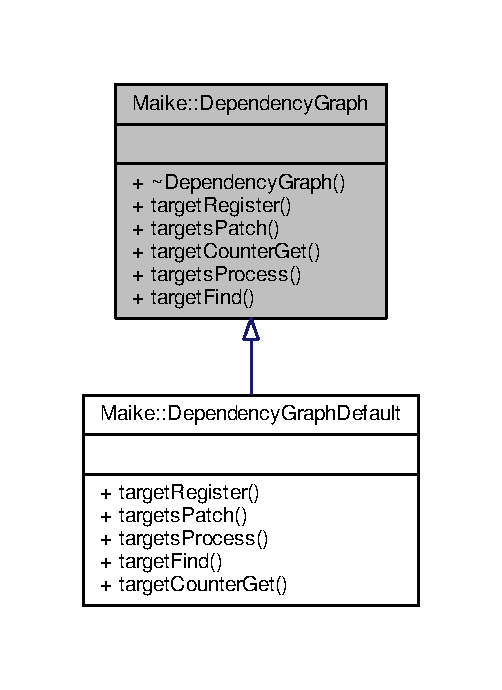
\includegraphics[width=241pt]{class_maike_1_1_dependency_graph__inherit__graph}
\end{center}
\end{figure}


Collaboration diagram for Maike\+:\+:Dependency\+Graph\+:\nopagebreak
\begin{figure}[H]
\begin{center}
\leavevmode
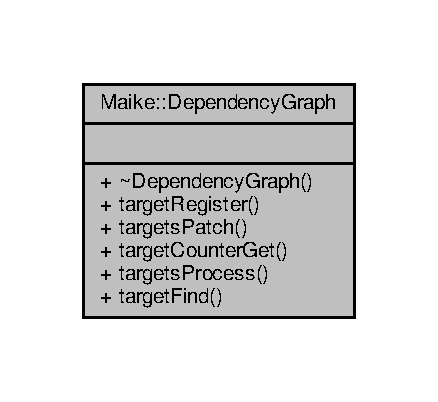
\includegraphics[width=210pt]{class_maike_1_1_dependency_graph__coll__graph}
\end{center}
\end{figure}
\subsection*{Classes}
\begin{DoxyCompactItemize}
\item 
class \hyperlink{class_maike_1_1_dependency_graph_1_1_target_processor}{Target\+Processor}
\end{DoxyCompactItemize}
\subsection*{Public Member Functions}
\begin{DoxyCompactItemize}
\item 
virtual \hyperlink{class_maike_1_1_dependency_graph_a1ebc7a3ae113077b51d87f59f8f8ec65}{$\sim$\+Dependency\+Graph} ()=default
\item 
virtual \hyperlink{class_maike_1_1_dependency_graph}{Dependency\+Graph} \& \hyperlink{class_maike_1_1_dependency_graph_a6c0c5e99fc930156123366b529310436}{target\+Register} (std\+::unique\+\_\+ptr$<$ \hyperlink{class_maike_1_1_target}{Target} $>$ \&\&target)=0
\item 
virtual \hyperlink{class_maike_1_1_dependency_graph}{Dependency\+Graph} \& \hyperlink{class_maike_1_1_dependency_graph_a49ac42d37065fd3c976e5ec9966816a8}{targets\+Patch} ()=0
\item 
virtual size\+\_\+t \hyperlink{class_maike_1_1_dependency_graph_a38f551d19ac653287bc12c6a449d44a0}{target\+Counter\+Get} () const noexcept=0
\item 
virtual \hyperlink{class_maike_1_1_dependency_graph}{Dependency\+Graph} \& \hyperlink{class_maike_1_1_dependency_graph_a8a9a603b3d0d7c62241510b8d59a9711}{targets\+Process} (\hyperlink{class_maike_1_1_dependency_graph_1_1_target_processor}{Target\+Processor} \&\&proc)=0
\item 
virtual \hyperlink{class_maike_1_1_target}{Target} $\ast$ \hyperlink{class_maike_1_1_dependency_graph_a45c5920ffc7b6500382171c700d9f6d4}{target\+Find} (const char $\ast$name)=0
\end{DoxyCompactItemize}


\subsection{Constructor \& Destructor Documentation}
\index{Maike\+::\+Dependency\+Graph@{Maike\+::\+Dependency\+Graph}!````~Dependency\+Graph@{$\sim$\+Dependency\+Graph}}
\index{````~Dependency\+Graph@{$\sim$\+Dependency\+Graph}!Maike\+::\+Dependency\+Graph@{Maike\+::\+Dependency\+Graph}}
\subsubsection[{\texorpdfstring{$\sim$\+Dependency\+Graph()=default}{~DependencyGraph()=default}}]{\setlength{\rightskip}{0pt plus 5cm}virtual Maike\+::\+Dependency\+Graph\+::$\sim$\+Dependency\+Graph (
\begin{DoxyParamCaption}
{}
\end{DoxyParamCaption}
)\hspace{0.3cm}{\ttfamily [virtual]}, {\ttfamily [default]}}\hypertarget{class_maike_1_1_dependency_graph_a1ebc7a3ae113077b51d87f59f8f8ec65}{}\label{class_maike_1_1_dependency_graph_a1ebc7a3ae113077b51d87f59f8f8ec65}


\subsection{Member Function Documentation}
\index{Maike\+::\+Dependency\+Graph@{Maike\+::\+Dependency\+Graph}!target\+Counter\+Get@{target\+Counter\+Get}}
\index{target\+Counter\+Get@{target\+Counter\+Get}!Maike\+::\+Dependency\+Graph@{Maike\+::\+Dependency\+Graph}}
\subsubsection[{\texorpdfstring{target\+Counter\+Get() const noexcept=0}{targetCounterGet() const noexcept=0}}]{\setlength{\rightskip}{0pt plus 5cm}virtual size\+\_\+t Maike\+::\+Dependency\+Graph\+::target\+Counter\+Get (
\begin{DoxyParamCaption}
{}
\end{DoxyParamCaption}
) const\hspace{0.3cm}{\ttfamily [pure virtual]}, {\ttfamily [noexcept]}}\hypertarget{class_maike_1_1_dependency_graph_a38f551d19ac653287bc12c6a449d44a0}{}\label{class_maike_1_1_dependency_graph_a38f551d19ac653287bc12c6a449d44a0}


Implemented in \hyperlink{class_maike_1_1_dependency_graph_default_afaba2cc265e1771f9743c03139c66531}{Maike\+::\+Dependency\+Graph\+Default}.

\index{Maike\+::\+Dependency\+Graph@{Maike\+::\+Dependency\+Graph}!target\+Find@{target\+Find}}
\index{target\+Find@{target\+Find}!Maike\+::\+Dependency\+Graph@{Maike\+::\+Dependency\+Graph}}
\subsubsection[{\texorpdfstring{target\+Find(const char $\ast$name)=0}{targetFind(const char *name)=0}}]{\setlength{\rightskip}{0pt plus 5cm}virtual {\bf Target}$\ast$ Maike\+::\+Dependency\+Graph\+::target\+Find (
\begin{DoxyParamCaption}
\item[{const char $\ast$}]{name}
\end{DoxyParamCaption}
)\hspace{0.3cm}{\ttfamily [pure virtual]}}\hypertarget{class_maike_1_1_dependency_graph_a45c5920ffc7b6500382171c700d9f6d4}{}\label{class_maike_1_1_dependency_graph_a45c5920ffc7b6500382171c700d9f6d4}


Implemented in \hyperlink{class_maike_1_1_dependency_graph_default_aa6f83242aa03c9d1141d896d6d120179}{Maike\+::\+Dependency\+Graph\+Default}.

\index{Maike\+::\+Dependency\+Graph@{Maike\+::\+Dependency\+Graph}!target\+Register@{target\+Register}}
\index{target\+Register@{target\+Register}!Maike\+::\+Dependency\+Graph@{Maike\+::\+Dependency\+Graph}}
\subsubsection[{\texorpdfstring{target\+Register(std\+::unique\+\_\+ptr$<$ Target $>$ \&\&target)=0}{targetRegister(std::unique_ptr< Target > &&target)=0}}]{\setlength{\rightskip}{0pt plus 5cm}virtual {\bf Dependency\+Graph}\& Maike\+::\+Dependency\+Graph\+::target\+Register (
\begin{DoxyParamCaption}
\item[{std\+::unique\+\_\+ptr$<$ {\bf Target} $>$ \&\&}]{target}
\end{DoxyParamCaption}
)\hspace{0.3cm}{\ttfamily [pure virtual]}}\hypertarget{class_maike_1_1_dependency_graph_a6c0c5e99fc930156123366b529310436}{}\label{class_maike_1_1_dependency_graph_a6c0c5e99fc930156123366b529310436}


Implemented in \hyperlink{class_maike_1_1_dependency_graph_default_a36a6b993ce9a0496b3af282fa84d0be2}{Maike\+::\+Dependency\+Graph\+Default}.

\index{Maike\+::\+Dependency\+Graph@{Maike\+::\+Dependency\+Graph}!targets\+Patch@{targets\+Patch}}
\index{targets\+Patch@{targets\+Patch}!Maike\+::\+Dependency\+Graph@{Maike\+::\+Dependency\+Graph}}
\subsubsection[{\texorpdfstring{targets\+Patch()=0}{targetsPatch()=0}}]{\setlength{\rightskip}{0pt plus 5cm}virtual {\bf Dependency\+Graph}\& Maike\+::\+Dependency\+Graph\+::targets\+Patch (
\begin{DoxyParamCaption}
{}
\end{DoxyParamCaption}
)\hspace{0.3cm}{\ttfamily [pure virtual]}}\hypertarget{class_maike_1_1_dependency_graph_a49ac42d37065fd3c976e5ec9966816a8}{}\label{class_maike_1_1_dependency_graph_a49ac42d37065fd3c976e5ec9966816a8}


Implemented in \hyperlink{class_maike_1_1_dependency_graph_default_ad4d840ced36a682f4b7da6d49dd139c1}{Maike\+::\+Dependency\+Graph\+Default}.

\index{Maike\+::\+Dependency\+Graph@{Maike\+::\+Dependency\+Graph}!targets\+Process@{targets\+Process}}
\index{targets\+Process@{targets\+Process}!Maike\+::\+Dependency\+Graph@{Maike\+::\+Dependency\+Graph}}
\subsubsection[{\texorpdfstring{targets\+Process(\+Target\+Processor \&\&proc)=0}{targetsProcess(TargetProcessor &&proc)=0}}]{\setlength{\rightskip}{0pt plus 5cm}virtual {\bf Dependency\+Graph}\& Maike\+::\+Dependency\+Graph\+::targets\+Process (
\begin{DoxyParamCaption}
\item[{{\bf Target\+Processor} \&\&}]{proc}
\end{DoxyParamCaption}
)\hspace{0.3cm}{\ttfamily [pure virtual]}}\hypertarget{class_maike_1_1_dependency_graph_a8a9a603b3d0d7c62241510b8d59a9711}{}\label{class_maike_1_1_dependency_graph_a8a9a603b3d0d7c62241510b8d59a9711}


Implemented in \hyperlink{class_maike_1_1_dependency_graph_default_ac669b8f05435f454c72cd256e66a0b2c}{Maike\+::\+Dependency\+Graph\+Default}.



The documentation for this class was generated from the following file\+:\begin{DoxyCompactItemize}
\item 
\hyperlink{dependencygraph_8hpp}{dependencygraph.\+hpp}\end{DoxyCompactItemize}

\hypertarget{class_maike_1_1_dependency_graph_default}{}\section{Maike\+:\+:Dependency\+Graph\+Default Class Reference}
\label{class_maike_1_1_dependency_graph_default}\index{Maike\+::\+Dependency\+Graph\+Default@{Maike\+::\+Dependency\+Graph\+Default}}


{\ttfamily \#include $<$dependencygraphdefault.\+hpp$>$}



Inheritance diagram for Maike\+:\+:Dependency\+Graph\+Default\+:\nopagebreak
\begin{figure}[H]
\begin{center}
\leavevmode
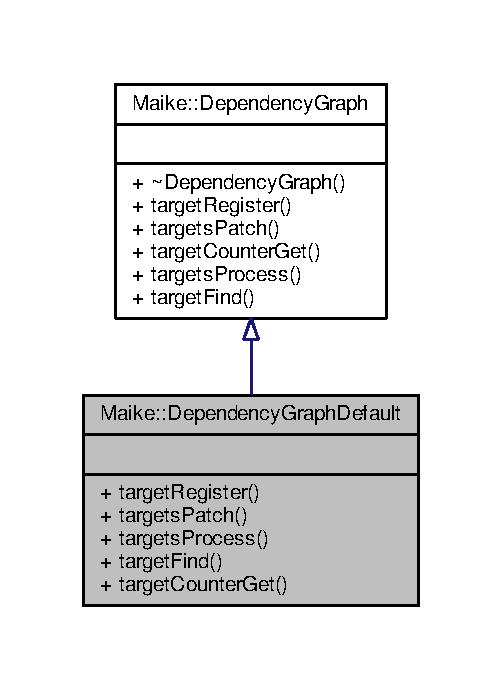
\includegraphics[width=241pt]{class_maike_1_1_dependency_graph_default__inherit__graph}
\end{center}
\end{figure}


Collaboration diagram for Maike\+:\+:Dependency\+Graph\+Default\+:\nopagebreak
\begin{figure}[H]
\begin{center}
\leavevmode
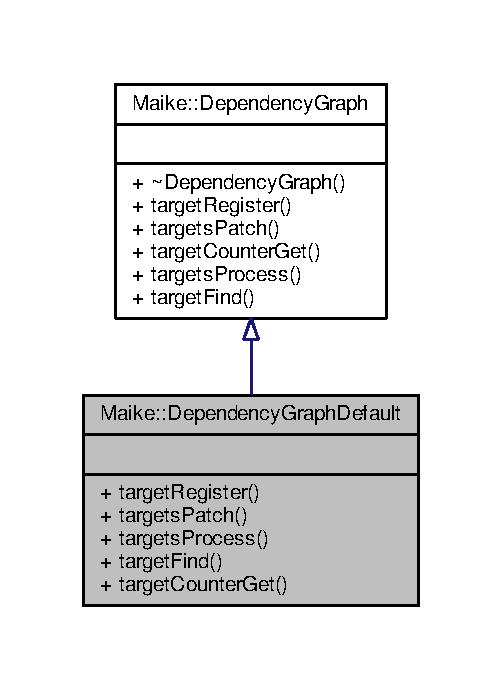
\includegraphics[width=241pt]{class_maike_1_1_dependency_graph_default__coll__graph}
\end{center}
\end{figure}
\subsection*{Public Member Functions}
\begin{DoxyCompactItemize}
\item 
\hyperlink{class_maike_1_1_dependency_graph_default}{Dependency\+Graph\+Default} \& \hyperlink{class_maike_1_1_dependency_graph_default_a36a6b993ce9a0496b3af282fa84d0be2}{target\+Register} (std\+::unique\+\_\+ptr$<$ \hyperlink{class_maike_1_1_target}{Target} $>$ \&\&target)
\item 
\hyperlink{class_maike_1_1_dependency_graph_default}{Dependency\+Graph\+Default} \& \hyperlink{class_maike_1_1_dependency_graph_default_ad4d840ced36a682f4b7da6d49dd139c1}{targets\+Patch} ()
\item 
\hyperlink{class_maike_1_1_dependency_graph_default}{Dependency\+Graph\+Default} \& \hyperlink{class_maike_1_1_dependency_graph_default_ac669b8f05435f454c72cd256e66a0b2c}{targets\+Process} (\hyperlink{class_maike_1_1_dependency_graph_1_1_target_processor}{Target\+Processor} \&\&visitor)
\item 
\hyperlink{class_maike_1_1_target}{Target} $\ast$ \hyperlink{class_maike_1_1_dependency_graph_default_aa6f83242aa03c9d1141d896d6d120179}{target\+Find} (const char $\ast$name)
\item 
size\+\_\+t \hyperlink{class_maike_1_1_dependency_graph_default_afaba2cc265e1771f9743c03139c66531}{target\+Counter\+Get} () const noexcept
\end{DoxyCompactItemize}


\subsection{Member Function Documentation}
\index{Maike\+::\+Dependency\+Graph\+Default@{Maike\+::\+Dependency\+Graph\+Default}!target\+Counter\+Get@{target\+Counter\+Get}}
\index{target\+Counter\+Get@{target\+Counter\+Get}!Maike\+::\+Dependency\+Graph\+Default@{Maike\+::\+Dependency\+Graph\+Default}}
\subsubsection[{\texorpdfstring{target\+Counter\+Get() const noexcept}{targetCounterGet() const noexcept}}]{\setlength{\rightskip}{0pt plus 5cm}size\+\_\+t Maike\+::\+Dependency\+Graph\+Default\+::target\+Counter\+Get (
\begin{DoxyParamCaption}
{}
\end{DoxyParamCaption}
) const\hspace{0.3cm}{\ttfamily [inline]}, {\ttfamily [virtual]}, {\ttfamily [noexcept]}}\hypertarget{class_maike_1_1_dependency_graph_default_afaba2cc265e1771f9743c03139c66531}{}\label{class_maike_1_1_dependency_graph_default_afaba2cc265e1771f9743c03139c66531}


Implements \hyperlink{class_maike_1_1_dependency_graph_a38f551d19ac653287bc12c6a449d44a0}{Maike\+::\+Dependency\+Graph}.

\index{Maike\+::\+Dependency\+Graph\+Default@{Maike\+::\+Dependency\+Graph\+Default}!target\+Find@{target\+Find}}
\index{target\+Find@{target\+Find}!Maike\+::\+Dependency\+Graph\+Default@{Maike\+::\+Dependency\+Graph\+Default}}
\subsubsection[{\texorpdfstring{target\+Find(const char $\ast$name)}{targetFind(const char *name)}}]{\setlength{\rightskip}{0pt plus 5cm}{\bf Target} $\ast$ Dependency\+Graph\+Default\+::target\+Find (
\begin{DoxyParamCaption}
\item[{const char $\ast$}]{name}
\end{DoxyParamCaption}
)\hspace{0.3cm}{\ttfamily [virtual]}}\hypertarget{class_maike_1_1_dependency_graph_default_aa6f83242aa03c9d1141d896d6d120179}{}\label{class_maike_1_1_dependency_graph_default_aa6f83242aa03c9d1141d896d6d120179}


Implements \hyperlink{class_maike_1_1_dependency_graph_a45c5920ffc7b6500382171c700d9f6d4}{Maike\+::\+Dependency\+Graph}.

\index{Maike\+::\+Dependency\+Graph\+Default@{Maike\+::\+Dependency\+Graph\+Default}!target\+Register@{target\+Register}}
\index{target\+Register@{target\+Register}!Maike\+::\+Dependency\+Graph\+Default@{Maike\+::\+Dependency\+Graph\+Default}}
\subsubsection[{\texorpdfstring{target\+Register(std\+::unique\+\_\+ptr$<$ Target $>$ \&\&target)}{targetRegister(std::unique_ptr< Target > &&target)}}]{\setlength{\rightskip}{0pt plus 5cm}{\bf Dependency\+Graph\+Default} \& Dependency\+Graph\+Default\+::target\+Register (
\begin{DoxyParamCaption}
\item[{std\+::unique\+\_\+ptr$<$ {\bf Target} $>$ \&\&}]{target}
\end{DoxyParamCaption}
)\hspace{0.3cm}{\ttfamily [virtual]}}\hypertarget{class_maike_1_1_dependency_graph_default_a36a6b993ce9a0496b3af282fa84d0be2}{}\label{class_maike_1_1_dependency_graph_default_a36a6b993ce9a0496b3af282fa84d0be2}


Implements \hyperlink{class_maike_1_1_dependency_graph_a6c0c5e99fc930156123366b529310436}{Maike\+::\+Dependency\+Graph}.

\index{Maike\+::\+Dependency\+Graph\+Default@{Maike\+::\+Dependency\+Graph\+Default}!targets\+Patch@{targets\+Patch}}
\index{targets\+Patch@{targets\+Patch}!Maike\+::\+Dependency\+Graph\+Default@{Maike\+::\+Dependency\+Graph\+Default}}
\subsubsection[{\texorpdfstring{targets\+Patch()}{targetsPatch()}}]{\setlength{\rightskip}{0pt plus 5cm}{\bf Dependency\+Graph\+Default} \& Dependency\+Graph\+Default\+::targets\+Patch (
\begin{DoxyParamCaption}
{}
\end{DoxyParamCaption}
)\hspace{0.3cm}{\ttfamily [virtual]}}\hypertarget{class_maike_1_1_dependency_graph_default_ad4d840ced36a682f4b7da6d49dd139c1}{}\label{class_maike_1_1_dependency_graph_default_ad4d840ced36a682f4b7da6d49dd139c1}


Implements \hyperlink{class_maike_1_1_dependency_graph_a49ac42d37065fd3c976e5ec9966816a8}{Maike\+::\+Dependency\+Graph}.

\index{Maike\+::\+Dependency\+Graph\+Default@{Maike\+::\+Dependency\+Graph\+Default}!targets\+Process@{targets\+Process}}
\index{targets\+Process@{targets\+Process}!Maike\+::\+Dependency\+Graph\+Default@{Maike\+::\+Dependency\+Graph\+Default}}
\subsubsection[{\texorpdfstring{targets\+Process(\+Target\+Processor \&\&visitor)}{targetsProcess(TargetProcessor &&visitor)}}]{\setlength{\rightskip}{0pt plus 5cm}{\bf Dependency\+Graph\+Default} \& Dependency\+Graph\+Default\+::targets\+Process (
\begin{DoxyParamCaption}
\item[{{\bf Target\+Processor} \&\&}]{visitor}
\end{DoxyParamCaption}
)\hspace{0.3cm}{\ttfamily [virtual]}}\hypertarget{class_maike_1_1_dependency_graph_default_ac669b8f05435f454c72cd256e66a0b2c}{}\label{class_maike_1_1_dependency_graph_default_ac669b8f05435f454c72cd256e66a0b2c}


Implements \hyperlink{class_maike_1_1_dependency_graph_a8a9a603b3d0d7c62241510b8d59a9711}{Maike\+::\+Dependency\+Graph}.



The documentation for this class was generated from the following files\+:\begin{DoxyCompactItemize}
\item 
\hyperlink{dependencygraphdefault_8hpp}{dependencygraphdefault.\+hpp}\item 
\hyperlink{dependencygraphdefault_8cpp}{dependencygraphdefault.\+cpp}\end{DoxyCompactItemize}

\hypertarget{class_maike_1_1_invoker}{}\section{Maike\+:\+:Invoker Class Reference}
\label{class_maike_1_1_invoker}\index{Maike\+::\+Invoker@{Maike\+::\+Invoker}}


{\ttfamily \#include $<$invoker.\+hpp$>$}



Inheritance diagram for Maike\+:\+:Invoker\+:\nopagebreak
\begin{figure}[H]
\begin{center}
\leavevmode
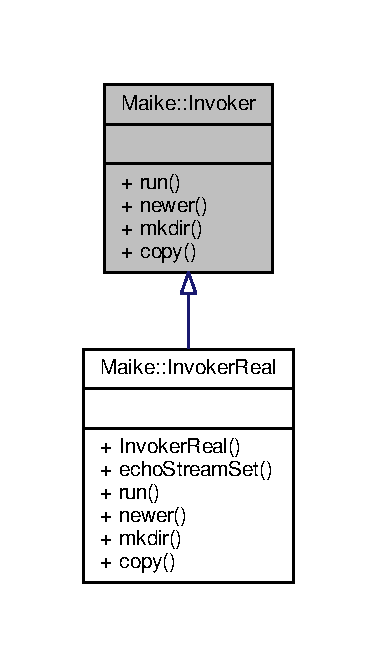
\includegraphics[width=181pt]{class_maike_1_1_invoker__inherit__graph}
\end{center}
\end{figure}


Collaboration diagram for Maike\+:\+:Invoker\+:\nopagebreak
\begin{figure}[H]
\begin{center}
\leavevmode
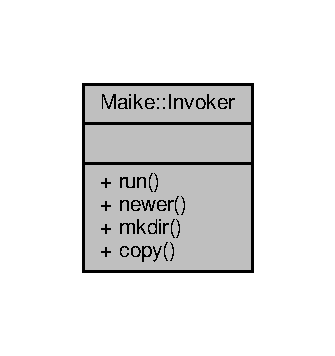
\includegraphics[width=161pt]{class_maike_1_1_invoker__coll__graph}
\end{center}
\end{figure}
\subsection*{Public Member Functions}
\begin{DoxyCompactItemize}
\item 
virtual void \hyperlink{class_maike_1_1_invoker_ac900f84da5bfa5a8e223f68c5d764f9c}{run} (const char $\ast$command, \hyperlink{struct_maike_1_1_twins}{Twins}$<$ const char $\ast$const $\ast$ $>$ args, Data\+Sink $\ast$standard\+\_\+output, Data\+Sink $\ast$standard\+\_\+error)=0
\item 
virtual bool \hyperlink{class_maike_1_1_invoker_abd35939892e10ae2b986029b6b465406}{newer} (const char $\ast$file\+\_\+a, const char $\ast$file\+\_\+b)=0
\item 
virtual void \hyperlink{class_maike_1_1_invoker_afe73fe8128cd90a03676944bd3e18379}{mkdir} (const char $\ast$name)=0
\item 
virtual void \hyperlink{class_maike_1_1_invoker_ab8b8e515508fa6c20b02d1d6cd0ac0d2}{copy} (const char $\ast$source, const char $\ast$dest)=0
\end{DoxyCompactItemize}


\subsection{Member Function Documentation}
\index{Maike\+::\+Invoker@{Maike\+::\+Invoker}!copy@{copy}}
\index{copy@{copy}!Maike\+::\+Invoker@{Maike\+::\+Invoker}}
\subsubsection[{\texorpdfstring{copy(const char $\ast$source, const char $\ast$dest)=0}{copy(const char *source, const char *dest)=0}}]{\setlength{\rightskip}{0pt plus 5cm}virtual void Maike\+::\+Invoker\+::copy (
\begin{DoxyParamCaption}
\item[{const char $\ast$}]{source, }
\item[{const char $\ast$}]{dest}
\end{DoxyParamCaption}
)\hspace{0.3cm}{\ttfamily [pure virtual]}}\hypertarget{class_maike_1_1_invoker_ab8b8e515508fa6c20b02d1d6cd0ac0d2}{}\label{class_maike_1_1_invoker_ab8b8e515508fa6c20b02d1d6cd0ac0d2}


Implemented in \hyperlink{class_maike_1_1_invoker_real_aaf83ba4c138e3c7c4f4c72d614972dcf}{Maike\+::\+Invoker\+Real}.

\index{Maike\+::\+Invoker@{Maike\+::\+Invoker}!mkdir@{mkdir}}
\index{mkdir@{mkdir}!Maike\+::\+Invoker@{Maike\+::\+Invoker}}
\subsubsection[{\texorpdfstring{mkdir(const char $\ast$name)=0}{mkdir(const char *name)=0}}]{\setlength{\rightskip}{0pt plus 5cm}virtual void Maike\+::\+Invoker\+::mkdir (
\begin{DoxyParamCaption}
\item[{const char $\ast$}]{name}
\end{DoxyParamCaption}
)\hspace{0.3cm}{\ttfamily [pure virtual]}}\hypertarget{class_maike_1_1_invoker_afe73fe8128cd90a03676944bd3e18379}{}\label{class_maike_1_1_invoker_afe73fe8128cd90a03676944bd3e18379}


Implemented in \hyperlink{class_maike_1_1_invoker_real_a1b36073b7647c0b454e20a1bfc48d1c0}{Maike\+::\+Invoker\+Real}.

\index{Maike\+::\+Invoker@{Maike\+::\+Invoker}!newer@{newer}}
\index{newer@{newer}!Maike\+::\+Invoker@{Maike\+::\+Invoker}}
\subsubsection[{\texorpdfstring{newer(const char $\ast$file\+\_\+a, const char $\ast$file\+\_\+b)=0}{newer(const char *file_a, const char *file_b)=0}}]{\setlength{\rightskip}{0pt plus 5cm}virtual bool Maike\+::\+Invoker\+::newer (
\begin{DoxyParamCaption}
\item[{const char $\ast$}]{file\+\_\+a, }
\item[{const char $\ast$}]{file\+\_\+b}
\end{DoxyParamCaption}
)\hspace{0.3cm}{\ttfamily [pure virtual]}}\hypertarget{class_maike_1_1_invoker_abd35939892e10ae2b986029b6b465406}{}\label{class_maike_1_1_invoker_abd35939892e10ae2b986029b6b465406}


Implemented in \hyperlink{class_maike_1_1_invoker_real_ab64b8508546174af514a1b78d2c7e9e6}{Maike\+::\+Invoker\+Real}.

\index{Maike\+::\+Invoker@{Maike\+::\+Invoker}!run@{run}}
\index{run@{run}!Maike\+::\+Invoker@{Maike\+::\+Invoker}}
\subsubsection[{\texorpdfstring{run(const char $\ast$command, Twins$<$ const char $\ast$const $\ast$ $>$ args, Data\+Sink $\ast$standard\+\_\+output, Data\+Sink $\ast$standard\+\_\+error)=0}{run(const char *command, Twins< const char *const * > args, DataSink *standard_output, DataSink *standard_error)=0}}]{\setlength{\rightskip}{0pt plus 5cm}virtual void Maike\+::\+Invoker\+::run (
\begin{DoxyParamCaption}
\item[{const char $\ast$}]{command, }
\item[{{\bf Twins}$<$ const char $\ast$const $\ast$ $>$}]{args, }
\item[{Data\+Sink $\ast$}]{standard\+\_\+output, }
\item[{Data\+Sink $\ast$}]{standard\+\_\+error}
\end{DoxyParamCaption}
)\hspace{0.3cm}{\ttfamily [pure virtual]}}\hypertarget{class_maike_1_1_invoker_ac900f84da5bfa5a8e223f68c5d764f9c}{}\label{class_maike_1_1_invoker_ac900f84da5bfa5a8e223f68c5d764f9c}


Implemented in \hyperlink{class_maike_1_1_invoker_real_a8d5109299e37127f09a010469dca1e33}{Maike\+::\+Invoker\+Real}.



The documentation for this class was generated from the following file\+:\begin{DoxyCompactItemize}
\item 
\hyperlink{invoker_8hpp}{invoker.\+hpp}\end{DoxyCompactItemize}

\hypertarget{class_maike_1_1_invoker_real}{}\section{Maike\+:\+:Invoker\+Real Class Reference}
\label{class_maike_1_1_invoker_real}\index{Maike\+::\+Invoker\+Real@{Maike\+::\+Invoker\+Real}}


{\ttfamily \#include $<$invokerreal.\+hpp$>$}



Inheritance diagram for Maike\+:\+:Invoker\+Real\+:\nopagebreak
\begin{figure}[H]
\begin{center}
\leavevmode
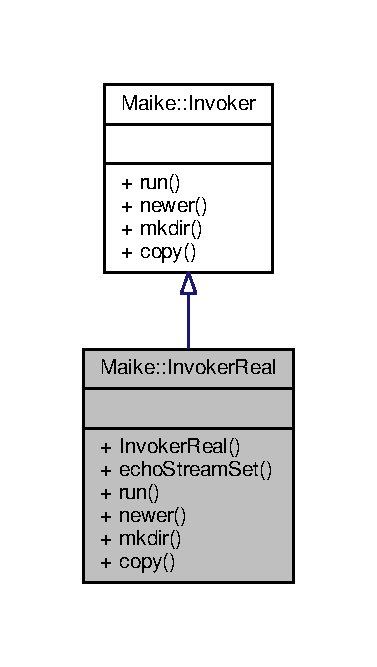
\includegraphics[width=181pt]{class_maike_1_1_invoker_real__inherit__graph}
\end{center}
\end{figure}


Collaboration diagram for Maike\+:\+:Invoker\+Real\+:\nopagebreak
\begin{figure}[H]
\begin{center}
\leavevmode
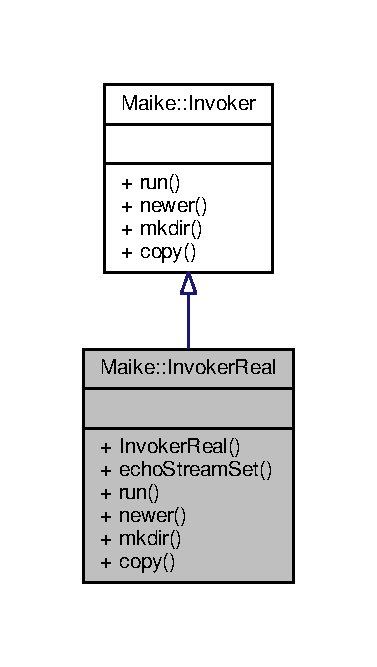
\includegraphics[width=181pt]{class_maike_1_1_invoker_real__coll__graph}
\end{center}
\end{figure}
\subsection*{Public Member Functions}
\begin{DoxyCompactItemize}
\item 
\hyperlink{class_maike_1_1_invoker_real_a51cf460d70fa46cbcb6a4b9f5e44f677}{Invoker\+Real} ()
\item 
\hyperlink{class_maike_1_1_invoker_real}{Invoker\+Real} \& \hyperlink{class_maike_1_1_invoker_real_adfeb0ba4cc7d7c8a2166396f3050d86b}{echo\+Stream\+Set} (Data\+Sink $\ast$sink) noexcept
\item 
void \hyperlink{class_maike_1_1_invoker_real_a8d5109299e37127f09a010469dca1e33}{run} (const char $\ast$command, \hyperlink{struct_maike_1_1_twins}{Twins}$<$ const char $\ast$const $\ast$ $>$ args, Data\+Sink $\ast$standard\+\_\+output, Data\+Sink $\ast$standard\+\_\+error)
\item 
bool \hyperlink{class_maike_1_1_invoker_real_ab64b8508546174af514a1b78d2c7e9e6}{newer} (const char $\ast$file\+\_\+a, const char $\ast$file\+\_\+b)
\item 
void \hyperlink{class_maike_1_1_invoker_real_a1b36073b7647c0b454e20a1bfc48d1c0}{mkdir} (const char $\ast$name)
\item 
void \hyperlink{class_maike_1_1_invoker_real_aaf83ba4c138e3c7c4f4c72d614972dcf}{copy} (const char $\ast$source, const char $\ast$dest)
\end{DoxyCompactItemize}


\subsection{Constructor \& Destructor Documentation}
\index{Maike\+::\+Invoker\+Real@{Maike\+::\+Invoker\+Real}!Invoker\+Real@{Invoker\+Real}}
\index{Invoker\+Real@{Invoker\+Real}!Maike\+::\+Invoker\+Real@{Maike\+::\+Invoker\+Real}}
\subsubsection[{\texorpdfstring{Invoker\+Real()}{InvokerReal()}}]{\setlength{\rightskip}{0pt plus 5cm}Maike\+::\+Invoker\+Real\+::\+Invoker\+Real (
\begin{DoxyParamCaption}
{}
\end{DoxyParamCaption}
)\hspace{0.3cm}{\ttfamily [inline]}}\hypertarget{class_maike_1_1_invoker_real_a51cf460d70fa46cbcb6a4b9f5e44f677}{}\label{class_maike_1_1_invoker_real_a51cf460d70fa46cbcb6a4b9f5e44f677}


\subsection{Member Function Documentation}
\index{Maike\+::\+Invoker\+Real@{Maike\+::\+Invoker\+Real}!copy@{copy}}
\index{copy@{copy}!Maike\+::\+Invoker\+Real@{Maike\+::\+Invoker\+Real}}
\subsubsection[{\texorpdfstring{copy(const char $\ast$source, const char $\ast$dest)}{copy(const char *source, const char *dest)}}]{\setlength{\rightskip}{0pt plus 5cm}void Maike\+::\+Invoker\+Real\+::copy (
\begin{DoxyParamCaption}
\item[{const char $\ast$}]{source, }
\item[{const char $\ast$}]{dest}
\end{DoxyParamCaption}
)\hspace{0.3cm}{\ttfamily [virtual]}}\hypertarget{class_maike_1_1_invoker_real_aaf83ba4c138e3c7c4f4c72d614972dcf}{}\label{class_maike_1_1_invoker_real_aaf83ba4c138e3c7c4f4c72d614972dcf}


Implements \hyperlink{class_maike_1_1_invoker_ab8b8e515508fa6c20b02d1d6cd0ac0d2}{Maike\+::\+Invoker}.

\index{Maike\+::\+Invoker\+Real@{Maike\+::\+Invoker\+Real}!echo\+Stream\+Set@{echo\+Stream\+Set}}
\index{echo\+Stream\+Set@{echo\+Stream\+Set}!Maike\+::\+Invoker\+Real@{Maike\+::\+Invoker\+Real}}
\subsubsection[{\texorpdfstring{echo\+Stream\+Set(\+Data\+Sink $\ast$sink) noexcept}{echoStreamSet(DataSink *sink) noexcept}}]{\setlength{\rightskip}{0pt plus 5cm}{\bf Invoker\+Real}\& Maike\+::\+Invoker\+Real\+::echo\+Stream\+Set (
\begin{DoxyParamCaption}
\item[{Data\+Sink $\ast$}]{sink}
\end{DoxyParamCaption}
)\hspace{0.3cm}{\ttfamily [inline]}, {\ttfamily [noexcept]}}\hypertarget{class_maike_1_1_invoker_real_adfeb0ba4cc7d7c8a2166396f3050d86b}{}\label{class_maike_1_1_invoker_real_adfeb0ba4cc7d7c8a2166396f3050d86b}
\index{Maike\+::\+Invoker\+Real@{Maike\+::\+Invoker\+Real}!mkdir@{mkdir}}
\index{mkdir@{mkdir}!Maike\+::\+Invoker\+Real@{Maike\+::\+Invoker\+Real}}
\subsubsection[{\texorpdfstring{mkdir(const char $\ast$name)}{mkdir(const char *name)}}]{\setlength{\rightskip}{0pt plus 5cm}void Maike\+::\+Invoker\+Real\+::mkdir (
\begin{DoxyParamCaption}
\item[{const char $\ast$}]{name}
\end{DoxyParamCaption}
)\hspace{0.3cm}{\ttfamily [virtual]}}\hypertarget{class_maike_1_1_invoker_real_a1b36073b7647c0b454e20a1bfc48d1c0}{}\label{class_maike_1_1_invoker_real_a1b36073b7647c0b454e20a1bfc48d1c0}


Implements \hyperlink{class_maike_1_1_invoker_afe73fe8128cd90a03676944bd3e18379}{Maike\+::\+Invoker}.

\index{Maike\+::\+Invoker\+Real@{Maike\+::\+Invoker\+Real}!newer@{newer}}
\index{newer@{newer}!Maike\+::\+Invoker\+Real@{Maike\+::\+Invoker\+Real}}
\subsubsection[{\texorpdfstring{newer(const char $\ast$file\+\_\+a, const char $\ast$file\+\_\+b)}{newer(const char *file_a, const char *file_b)}}]{\setlength{\rightskip}{0pt plus 5cm}bool Maike\+::\+Invoker\+Real\+::newer (
\begin{DoxyParamCaption}
\item[{const char $\ast$}]{file\+\_\+a, }
\item[{const char $\ast$}]{file\+\_\+b}
\end{DoxyParamCaption}
)\hspace{0.3cm}{\ttfamily [virtual]}}\hypertarget{class_maike_1_1_invoker_real_ab64b8508546174af514a1b78d2c7e9e6}{}\label{class_maike_1_1_invoker_real_ab64b8508546174af514a1b78d2c7e9e6}


Implements \hyperlink{class_maike_1_1_invoker_abd35939892e10ae2b986029b6b465406}{Maike\+::\+Invoker}.

\index{Maike\+::\+Invoker\+Real@{Maike\+::\+Invoker\+Real}!run@{run}}
\index{run@{run}!Maike\+::\+Invoker\+Real@{Maike\+::\+Invoker\+Real}}
\subsubsection[{\texorpdfstring{run(const char $\ast$command, Twins$<$ const char $\ast$const $\ast$ $>$ args, Data\+Sink $\ast$standard\+\_\+output, Data\+Sink $\ast$standard\+\_\+error)}{run(const char *command, Twins< const char *const * > args, DataSink *standard_output, DataSink *standard_error)}}]{\setlength{\rightskip}{0pt plus 5cm}void Maike\+::\+Invoker\+Real\+::run (
\begin{DoxyParamCaption}
\item[{const char $\ast$}]{command, }
\item[{{\bf Twins}$<$ const char $\ast$const $\ast$ $>$}]{args, }
\item[{Data\+Sink $\ast$}]{standard\+\_\+output, }
\item[{Data\+Sink $\ast$}]{standard\+\_\+error}
\end{DoxyParamCaption}
)\hspace{0.3cm}{\ttfamily [virtual]}}\hypertarget{class_maike_1_1_invoker_real_a8d5109299e37127f09a010469dca1e33}{}\label{class_maike_1_1_invoker_real_a8d5109299e37127f09a010469dca1e33}


Implements \hyperlink{class_maike_1_1_invoker_ac900f84da5bfa5a8e223f68c5d764f9c}{Maike\+::\+Invoker}.



The documentation for this class was generated from the following file\+:\begin{DoxyCompactItemize}
\item 
\hyperlink{invokerreal_8hpp}{invokerreal.\+hpp}\end{DoxyCompactItemize}

\hypertarget{class_leaf_collector}{}\section{Leaf\+Collector Class Reference}
\label{class_leaf_collector}\index{Leaf\+Collector@{Leaf\+Collector}}


Inheritance diagram for Leaf\+Collector\+:\nopagebreak
\begin{figure}[H]
\begin{center}
\leavevmode
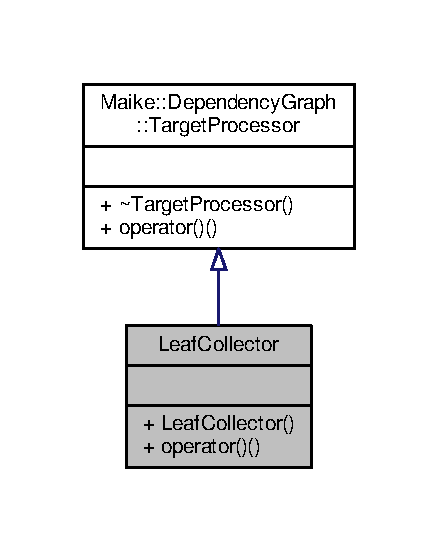
\includegraphics[width=210pt]{class_leaf_collector__inherit__graph}
\end{center}
\end{figure}


Collaboration diagram for Leaf\+Collector\+:\nopagebreak
\begin{figure}[H]
\begin{center}
\leavevmode
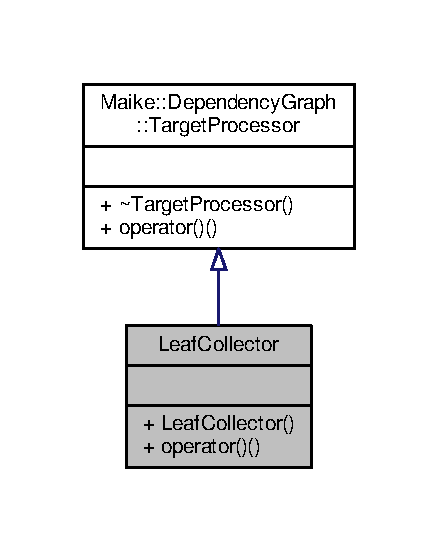
\includegraphics[width=210pt]{class_leaf_collector__coll__graph}
\end{center}
\end{figure}
\subsection*{Public Member Functions}
\begin{DoxyCompactItemize}
\item 
\hyperlink{class_leaf_collector_ae4a3985e6c3729bdd1d5475ee6251fba}{Leaf\+Collector} (std\+::vector$<$ \hyperlink{class_maike_1_1_target}{Maike\+::\+Target} $\ast$ $>$ \&leafs)
\item 
void \hyperlink{class_leaf_collector_ad6eefbdbcf3710390449fab9aa8dfbfb}{operator()} (\hyperlink{class_maike_1_1_dependency_graph}{Maike\+::\+Dependency\+Graph} \&graph, \hyperlink{class_maike_1_1_target}{Maike\+::\+Target} \&target\+\_\+current)
\end{DoxyCompactItemize}


\subsection{Constructor \& Destructor Documentation}
\index{Leaf\+Collector@{Leaf\+Collector}!Leaf\+Collector@{Leaf\+Collector}}
\index{Leaf\+Collector@{Leaf\+Collector}!Leaf\+Collector@{Leaf\+Collector}}
\subsubsection[{\texorpdfstring{Leaf\+Collector(std\+::vector$<$ Maike\+::\+Target $\ast$ $>$ \&leafs)}{LeafCollector(std::vector< Maike::Target * > &leafs)}}]{\setlength{\rightskip}{0pt plus 5cm}Leaf\+Collector\+::\+Leaf\+Collector (
\begin{DoxyParamCaption}
\item[{std\+::vector$<$ {\bf Maike\+::\+Target} $\ast$ $>$ \&}]{leafs}
\end{DoxyParamCaption}
)\hspace{0.3cm}{\ttfamily [inline]}}\hypertarget{class_leaf_collector_ae4a3985e6c3729bdd1d5475ee6251fba}{}\label{class_leaf_collector_ae4a3985e6c3729bdd1d5475ee6251fba}


\subsection{Member Function Documentation}
\index{Leaf\+Collector@{Leaf\+Collector}!operator()@{operator()}}
\index{operator()@{operator()}!Leaf\+Collector@{Leaf\+Collector}}
\subsubsection[{\texorpdfstring{operator()(\+Maike\+::\+Dependency\+Graph \&graph, Maike\+::\+Target \&target\+\_\+current)}{operator()(Maike::DependencyGraph &graph, Maike::Target &target_current)}}]{\setlength{\rightskip}{0pt plus 5cm}void Leaf\+Collector\+::operator() (
\begin{DoxyParamCaption}
\item[{{\bf Maike\+::\+Dependency\+Graph} \&}]{graph, }
\item[{{\bf Maike\+::\+Target} \&}]{target\+\_\+current}
\end{DoxyParamCaption}
)\hspace{0.3cm}{\ttfamily [inline]}, {\ttfamily [virtual]}}\hypertarget{class_leaf_collector_ad6eefbdbcf3710390449fab9aa8dfbfb}{}\label{class_leaf_collector_ad6eefbdbcf3710390449fab9aa8dfbfb}


Implements \hyperlink{class_maike_1_1_dependency_graph_1_1_target_processor_af9bbe41827153c1bcbb01c62423a7850}{Maike\+::\+Dependency\+Graph\+::\+Target\+Processor}.



The documentation for this class was generated from the following file\+:\begin{DoxyCompactItemize}
\item 
\hyperlink{maike-main_8cpp}{maike-\/main.\+cpp}\end{DoxyCompactItemize}

\hypertarget{class_maike_1_1_spider}{}\section{Maike\+:\+:Spider Class Reference}
\label{class_maike_1_1_spider}\index{Maike\+::\+Spider@{Maike\+::\+Spider}}


{\ttfamily \#include $<$spider.\+hpp$>$}



Collaboration diagram for Maike\+:\+:Spider\+:\nopagebreak
\begin{figure}[H]
\begin{center}
\leavevmode
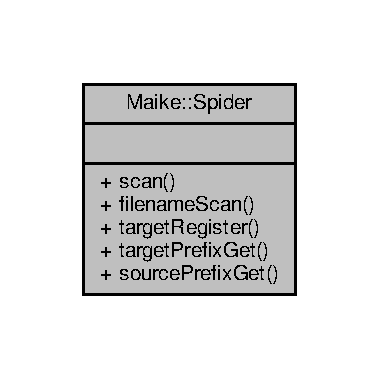
\includegraphics[width=182pt]{class_maike_1_1_spider__coll__graph}
\end{center}
\end{figure}
\subsection*{Public Member Functions}
\begin{DoxyCompactItemize}
\item 
virtual \hyperlink{class_maike_1_1_spider}{Spider} \& \hyperlink{class_maike_1_1_spider_aae962c763a5e8541c93661487fc7d99a}{scan} (const char $\ast$directory)=0
\item 
virtual \hyperlink{class_maike_1_1_spider}{Spider} \& \hyperlink{class_maike_1_1_spider_a548a255dacdd298d93a53537283404f4}{filename\+Scan} (const char $\ast$filename)=0
\item 
virtual \hyperlink{class_maike_1_1_spider}{Spider} \& \hyperlink{class_maike_1_1_spider_af28c61e85a9b9235d957cb8641b99648}{target\+Register} (std\+::unique\+\_\+ptr$<$ \hyperlink{class_maike_1_1_target}{Target} $>$ \&\&target)=0
\item 
virtual const char $\ast$ \hyperlink{class_maike_1_1_spider_a9b0d76b47e9aab5d69cd5aac08e77a85}{target\+Prefix\+Get} () const noexcept=0
\item 
virtual const char $\ast$ \hyperlink{class_maike_1_1_spider_a0376d7b089a79cbb31d15d5fe7d17650}{source\+Prefix\+Get} () const noexcept=0
\end{DoxyCompactItemize}


\subsection{Member Function Documentation}
\index{Maike\+::\+Spider@{Maike\+::\+Spider}!filename\+Scan@{filename\+Scan}}
\index{filename\+Scan@{filename\+Scan}!Maike\+::\+Spider@{Maike\+::\+Spider}}
\subsubsection[{\texorpdfstring{filename\+Scan(const char $\ast$filename)=0}{filenameScan(const char *filename)=0}}]{\setlength{\rightskip}{0pt plus 5cm}virtual {\bf Spider}\& Maike\+::\+Spider\+::filename\+Scan (
\begin{DoxyParamCaption}
\item[{const char $\ast$}]{filename}
\end{DoxyParamCaption}
)\hspace{0.3cm}{\ttfamily [pure virtual]}}\hypertarget{class_maike_1_1_spider_a548a255dacdd298d93a53537283404f4}{}\label{class_maike_1_1_spider_a548a255dacdd298d93a53537283404f4}
\index{Maike\+::\+Spider@{Maike\+::\+Spider}!scan@{scan}}
\index{scan@{scan}!Maike\+::\+Spider@{Maike\+::\+Spider}}
\subsubsection[{\texorpdfstring{scan(const char $\ast$directory)=0}{scan(const char *directory)=0}}]{\setlength{\rightskip}{0pt plus 5cm}virtual {\bf Spider}\& Maike\+::\+Spider\+::scan (
\begin{DoxyParamCaption}
\item[{const char $\ast$}]{directory}
\end{DoxyParamCaption}
)\hspace{0.3cm}{\ttfamily [pure virtual]}}\hypertarget{class_maike_1_1_spider_aae962c763a5e8541c93661487fc7d99a}{}\label{class_maike_1_1_spider_aae962c763a5e8541c93661487fc7d99a}
\index{Maike\+::\+Spider@{Maike\+::\+Spider}!source\+Prefix\+Get@{source\+Prefix\+Get}}
\index{source\+Prefix\+Get@{source\+Prefix\+Get}!Maike\+::\+Spider@{Maike\+::\+Spider}}
\subsubsection[{\texorpdfstring{source\+Prefix\+Get() const noexcept=0}{sourcePrefixGet() const noexcept=0}}]{\setlength{\rightskip}{0pt plus 5cm}virtual const char$\ast$ Maike\+::\+Spider\+::source\+Prefix\+Get (
\begin{DoxyParamCaption}
{}
\end{DoxyParamCaption}
) const\hspace{0.3cm}{\ttfamily [pure virtual]}, {\ttfamily [noexcept]}}\hypertarget{class_maike_1_1_spider_a0376d7b089a79cbb31d15d5fe7d17650}{}\label{class_maike_1_1_spider_a0376d7b089a79cbb31d15d5fe7d17650}
\index{Maike\+::\+Spider@{Maike\+::\+Spider}!target\+Prefix\+Get@{target\+Prefix\+Get}}
\index{target\+Prefix\+Get@{target\+Prefix\+Get}!Maike\+::\+Spider@{Maike\+::\+Spider}}
\subsubsection[{\texorpdfstring{target\+Prefix\+Get() const noexcept=0}{targetPrefixGet() const noexcept=0}}]{\setlength{\rightskip}{0pt plus 5cm}virtual const char$\ast$ Maike\+::\+Spider\+::target\+Prefix\+Get (
\begin{DoxyParamCaption}
{}
\end{DoxyParamCaption}
) const\hspace{0.3cm}{\ttfamily [pure virtual]}, {\ttfamily [noexcept]}}\hypertarget{class_maike_1_1_spider_a9b0d76b47e9aab5d69cd5aac08e77a85}{}\label{class_maike_1_1_spider_a9b0d76b47e9aab5d69cd5aac08e77a85}
\index{Maike\+::\+Spider@{Maike\+::\+Spider}!target\+Register@{target\+Register}}
\index{target\+Register@{target\+Register}!Maike\+::\+Spider@{Maike\+::\+Spider}}
\subsubsection[{\texorpdfstring{target\+Register(std\+::unique\+\_\+ptr$<$ Target $>$ \&\&target)=0}{targetRegister(std::unique_ptr< Target > &&target)=0}}]{\setlength{\rightskip}{0pt plus 5cm}virtual {\bf Spider}\& Maike\+::\+Spider\+::target\+Register (
\begin{DoxyParamCaption}
\item[{std\+::unique\+\_\+ptr$<$ {\bf Target} $>$ \&\&}]{target}
\end{DoxyParamCaption}
)\hspace{0.3cm}{\ttfamily [pure virtual]}}\hypertarget{class_maike_1_1_spider_af28c61e85a9b9235d957cb8641b99648}{}\label{class_maike_1_1_spider_af28c61e85a9b9235d957cb8641b99648}


The documentation for this class was generated from the following file\+:\begin{DoxyCompactItemize}
\item 
\hyperlink{spider_8hpp}{spider.\+hpp}\end{DoxyCompactItemize}

\hypertarget{class_maike_1_1_target}{}\section{Maike\+:\+:Target Class Reference}
\label{class_maike_1_1_target}\index{Maike\+::\+Target@{Maike\+::\+Target}}


{\ttfamily \#include $<$target.\+hpp$>$}



Collaboration diagram for Maike\+:\+:Target\+:\nopagebreak
\begin{figure}[H]
\begin{center}
\leavevmode
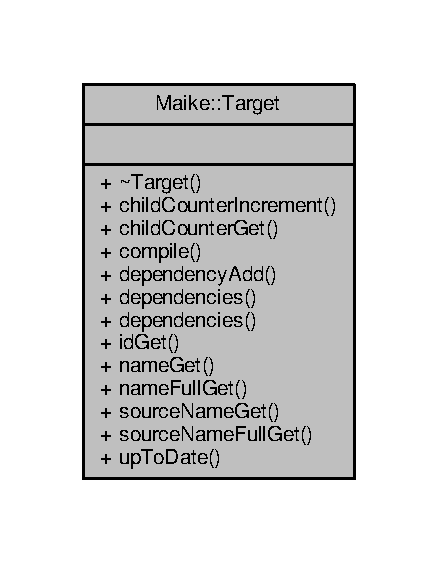
\includegraphics[width=210pt]{class_maike_1_1_target__coll__graph}
\end{center}
\end{figure}
\subsection*{Public Member Functions}
\begin{DoxyCompactItemize}
\item 
virtual \hyperlink{class_maike_1_1_target_aa2d6b53a7655c6daef570062a63bcabf}{$\sim$\+Target} ()=default
\item 
virtual \hyperlink{class_maike_1_1_target}{Target} \& \hyperlink{class_maike_1_1_target_a36c0f490a869e438b8a24c55d544aac2}{child\+Counter\+Increment} () noexcept=0
\item 
virtual size\+\_\+t \hyperlink{class_maike_1_1_target_a9ab02f5632d53552e6b6fc554151b0fb}{child\+Counter\+Get} () const noexcept=0
\item 
virtual bool \hyperlink{class_maike_1_1_target_a6f8fb0e12684b7c699e4cd1f16a5c35f}{compile} (\hyperlink{struct_maike_1_1_twins}{Twins}$<$ const \hyperlink{class_maike_1_1_dependency}{Dependency} $\ast$ $>$ dependency\+\_\+list, \hyperlink{class_maike_1_1_invoker}{Invoker} \&invoker) noexcept=0
\item 
virtual void \hyperlink{class_maike_1_1_target_a901b82d44e48d2050bc9107f3bc31348}{dependency\+Add} (\hyperlink{class_maike_1_1_dependency}{Dependency} \&\&dep)=0
\item 
virtual \hyperlink{struct_maike_1_1_twins}{Twins}$<$ const \hyperlink{class_maike_1_1_dependency}{Dependency} $\ast$ $>$ \hyperlink{class_maike_1_1_target_aca2d8c784e9f1ee8527b361dda109a20}{dependencies} () const noexcept=0
\item 
virtual \hyperlink{struct_maike_1_1_twins}{Twins}$<$ \hyperlink{class_maike_1_1_dependency}{Dependency} $\ast$ $>$ \hyperlink{class_maike_1_1_target_a5e22273131ace8711219f2edf7e69a72}{dependencies} () noexcept=0
\item 
virtual size\+\_\+t \hyperlink{class_maike_1_1_target_a8a8ee23dcb3c1ec7a674d8eed67233d5}{id\+Get} () const noexcept=0
\item 
virtual const char $\ast$ \hyperlink{class_maike_1_1_target_ad68cea274bfcaef5cc99b7671f92be17}{name\+Get} () const noexcept=0
\item 
virtual const char $\ast$ \hyperlink{class_maike_1_1_target_a38c1d42dd42ae141310df41ebd5b71fc}{name\+Full\+Get} () const noexcept=0
\item 
virtual const char $\ast$ \hyperlink{class_maike_1_1_target_a92a08944fb8ab1fe745cb4bdf1f15acb}{source\+Name\+Get} () const noexcept=0
\item 
virtual const char $\ast$ \hyperlink{class_maike_1_1_target_a1a851256ee2e022b1491c2c91e88a4ad}{source\+Name\+Full\+Get} () const noexcept=0
\item 
virtual bool \hyperlink{class_maike_1_1_target_a893976cd47a84706bdcb3b69a9f068ad}{up\+To\+Date} (\hyperlink{struct_maike_1_1_twins}{Twins}$<$ const \hyperlink{class_maike_1_1_dependency}{Dependency} $\ast$ $>$ dependency\+\_\+list, \hyperlink{class_maike_1_1_invoker}{Invoker} \&invoker) const noexcept=0
\end{DoxyCompactItemize}


\subsection{Constructor \& Destructor Documentation}
\index{Maike\+::\+Target@{Maike\+::\+Target}!````~Target@{$\sim$\+Target}}
\index{````~Target@{$\sim$\+Target}!Maike\+::\+Target@{Maike\+::\+Target}}
\subsubsection[{\texorpdfstring{$\sim$\+Target()=default}{~Target()=default}}]{\setlength{\rightskip}{0pt plus 5cm}virtual Maike\+::\+Target\+::$\sim$\+Target (
\begin{DoxyParamCaption}
{}
\end{DoxyParamCaption}
)\hspace{0.3cm}{\ttfamily [virtual]}, {\ttfamily [default]}}\hypertarget{class_maike_1_1_target_aa2d6b53a7655c6daef570062a63bcabf}{}\label{class_maike_1_1_target_aa2d6b53a7655c6daef570062a63bcabf}


\subsection{Member Function Documentation}
\index{Maike\+::\+Target@{Maike\+::\+Target}!child\+Counter\+Get@{child\+Counter\+Get}}
\index{child\+Counter\+Get@{child\+Counter\+Get}!Maike\+::\+Target@{Maike\+::\+Target}}
\subsubsection[{\texorpdfstring{child\+Counter\+Get() const noexcept=0}{childCounterGet() const noexcept=0}}]{\setlength{\rightskip}{0pt plus 5cm}virtual size\+\_\+t Maike\+::\+Target\+::child\+Counter\+Get (
\begin{DoxyParamCaption}
{}
\end{DoxyParamCaption}
) const\hspace{0.3cm}{\ttfamily [pure virtual]}, {\ttfamily [noexcept]}}\hypertarget{class_maike_1_1_target_a9ab02f5632d53552e6b6fc554151b0fb}{}\label{class_maike_1_1_target_a9ab02f5632d53552e6b6fc554151b0fb}
\index{Maike\+::\+Target@{Maike\+::\+Target}!child\+Counter\+Increment@{child\+Counter\+Increment}}
\index{child\+Counter\+Increment@{child\+Counter\+Increment}!Maike\+::\+Target@{Maike\+::\+Target}}
\subsubsection[{\texorpdfstring{child\+Counter\+Increment() noexcept=0}{childCounterIncrement() noexcept=0}}]{\setlength{\rightskip}{0pt plus 5cm}virtual {\bf Target}\& Maike\+::\+Target\+::child\+Counter\+Increment (
\begin{DoxyParamCaption}
{}
\end{DoxyParamCaption}
)\hspace{0.3cm}{\ttfamily [pure virtual]}, {\ttfamily [noexcept]}}\hypertarget{class_maike_1_1_target_a36c0f490a869e438b8a24c55d544aac2}{}\label{class_maike_1_1_target_a36c0f490a869e438b8a24c55d544aac2}
\index{Maike\+::\+Target@{Maike\+::\+Target}!compile@{compile}}
\index{compile@{compile}!Maike\+::\+Target@{Maike\+::\+Target}}
\subsubsection[{\texorpdfstring{compile(\+Twins$<$ const Dependency $\ast$ $>$ dependency\+\_\+list, Invoker \&invoker) noexcept=0}{compile(Twins< const Dependency * > dependency_list, Invoker &invoker) noexcept=0}}]{\setlength{\rightskip}{0pt plus 5cm}virtual bool Maike\+::\+Target\+::compile (
\begin{DoxyParamCaption}
\item[{{\bf Twins}$<$ const {\bf Dependency} $\ast$ $>$}]{dependency\+\_\+list, }
\item[{{\bf Invoker} \&}]{invoker}
\end{DoxyParamCaption}
)\hspace{0.3cm}{\ttfamily [pure virtual]}, {\ttfamily [noexcept]}}\hypertarget{class_maike_1_1_target_a6f8fb0e12684b7c699e4cd1f16a5c35f}{}\label{class_maike_1_1_target_a6f8fb0e12684b7c699e4cd1f16a5c35f}
\index{Maike\+::\+Target@{Maike\+::\+Target}!dependencies@{dependencies}}
\index{dependencies@{dependencies}!Maike\+::\+Target@{Maike\+::\+Target}}
\subsubsection[{\texorpdfstring{dependencies() const noexcept=0}{dependencies() const noexcept=0}}]{\setlength{\rightskip}{0pt plus 5cm}virtual {\bf Twins}$<$const {\bf Dependency}$\ast$$>$ Maike\+::\+Target\+::dependencies (
\begin{DoxyParamCaption}
{}
\end{DoxyParamCaption}
) const\hspace{0.3cm}{\ttfamily [pure virtual]}, {\ttfamily [noexcept]}}\hypertarget{class_maike_1_1_target_aca2d8c784e9f1ee8527b361dda109a20}{}\label{class_maike_1_1_target_aca2d8c784e9f1ee8527b361dda109a20}
\index{Maike\+::\+Target@{Maike\+::\+Target}!dependencies@{dependencies}}
\index{dependencies@{dependencies}!Maike\+::\+Target@{Maike\+::\+Target}}
\subsubsection[{\texorpdfstring{dependencies() noexcept=0}{dependencies() noexcept=0}}]{\setlength{\rightskip}{0pt plus 5cm}virtual {\bf Twins}$<${\bf Dependency}$\ast$$>$ Maike\+::\+Target\+::dependencies (
\begin{DoxyParamCaption}
{}
\end{DoxyParamCaption}
)\hspace{0.3cm}{\ttfamily [pure virtual]}, {\ttfamily [noexcept]}}\hypertarget{class_maike_1_1_target_a5e22273131ace8711219f2edf7e69a72}{}\label{class_maike_1_1_target_a5e22273131ace8711219f2edf7e69a72}
\index{Maike\+::\+Target@{Maike\+::\+Target}!dependency\+Add@{dependency\+Add}}
\index{dependency\+Add@{dependency\+Add}!Maike\+::\+Target@{Maike\+::\+Target}}
\subsubsection[{\texorpdfstring{dependency\+Add(\+Dependency \&\&dep)=0}{dependencyAdd(Dependency &&dep)=0}}]{\setlength{\rightskip}{0pt plus 5cm}virtual void Maike\+::\+Target\+::dependency\+Add (
\begin{DoxyParamCaption}
\item[{{\bf Dependency} \&\&}]{dep}
\end{DoxyParamCaption}
)\hspace{0.3cm}{\ttfamily [pure virtual]}}\hypertarget{class_maike_1_1_target_a901b82d44e48d2050bc9107f3bc31348}{}\label{class_maike_1_1_target_a901b82d44e48d2050bc9107f3bc31348}
\index{Maike\+::\+Target@{Maike\+::\+Target}!id\+Get@{id\+Get}}
\index{id\+Get@{id\+Get}!Maike\+::\+Target@{Maike\+::\+Target}}
\subsubsection[{\texorpdfstring{id\+Get() const noexcept=0}{idGet() const noexcept=0}}]{\setlength{\rightskip}{0pt plus 5cm}virtual size\+\_\+t Maike\+::\+Target\+::id\+Get (
\begin{DoxyParamCaption}
{}
\end{DoxyParamCaption}
) const\hspace{0.3cm}{\ttfamily [pure virtual]}, {\ttfamily [noexcept]}}\hypertarget{class_maike_1_1_target_a8a8ee23dcb3c1ec7a674d8eed67233d5}{}\label{class_maike_1_1_target_a8a8ee23dcb3c1ec7a674d8eed67233d5}
\index{Maike\+::\+Target@{Maike\+::\+Target}!name\+Full\+Get@{name\+Full\+Get}}
\index{name\+Full\+Get@{name\+Full\+Get}!Maike\+::\+Target@{Maike\+::\+Target}}
\subsubsection[{\texorpdfstring{name\+Full\+Get() const noexcept=0}{nameFullGet() const noexcept=0}}]{\setlength{\rightskip}{0pt plus 5cm}virtual const char$\ast$ Maike\+::\+Target\+::name\+Full\+Get (
\begin{DoxyParamCaption}
{}
\end{DoxyParamCaption}
) const\hspace{0.3cm}{\ttfamily [pure virtual]}, {\ttfamily [noexcept]}}\hypertarget{class_maike_1_1_target_a38c1d42dd42ae141310df41ebd5b71fc}{}\label{class_maike_1_1_target_a38c1d42dd42ae141310df41ebd5b71fc}
\index{Maike\+::\+Target@{Maike\+::\+Target}!name\+Get@{name\+Get}}
\index{name\+Get@{name\+Get}!Maike\+::\+Target@{Maike\+::\+Target}}
\subsubsection[{\texorpdfstring{name\+Get() const noexcept=0}{nameGet() const noexcept=0}}]{\setlength{\rightskip}{0pt plus 5cm}virtual const char$\ast$ Maike\+::\+Target\+::name\+Get (
\begin{DoxyParamCaption}
{}
\end{DoxyParamCaption}
) const\hspace{0.3cm}{\ttfamily [pure virtual]}, {\ttfamily [noexcept]}}\hypertarget{class_maike_1_1_target_ad68cea274bfcaef5cc99b7671f92be17}{}\label{class_maike_1_1_target_ad68cea274bfcaef5cc99b7671f92be17}
\index{Maike\+::\+Target@{Maike\+::\+Target}!source\+Name\+Full\+Get@{source\+Name\+Full\+Get}}
\index{source\+Name\+Full\+Get@{source\+Name\+Full\+Get}!Maike\+::\+Target@{Maike\+::\+Target}}
\subsubsection[{\texorpdfstring{source\+Name\+Full\+Get() const noexcept=0}{sourceNameFullGet() const noexcept=0}}]{\setlength{\rightskip}{0pt plus 5cm}virtual const char$\ast$ Maike\+::\+Target\+::source\+Name\+Full\+Get (
\begin{DoxyParamCaption}
{}
\end{DoxyParamCaption}
) const\hspace{0.3cm}{\ttfamily [pure virtual]}, {\ttfamily [noexcept]}}\hypertarget{class_maike_1_1_target_a1a851256ee2e022b1491c2c91e88a4ad}{}\label{class_maike_1_1_target_a1a851256ee2e022b1491c2c91e88a4ad}
\index{Maike\+::\+Target@{Maike\+::\+Target}!source\+Name\+Get@{source\+Name\+Get}}
\index{source\+Name\+Get@{source\+Name\+Get}!Maike\+::\+Target@{Maike\+::\+Target}}
\subsubsection[{\texorpdfstring{source\+Name\+Get() const noexcept=0}{sourceNameGet() const noexcept=0}}]{\setlength{\rightskip}{0pt plus 5cm}virtual const char$\ast$ Maike\+::\+Target\+::source\+Name\+Get (
\begin{DoxyParamCaption}
{}
\end{DoxyParamCaption}
) const\hspace{0.3cm}{\ttfamily [pure virtual]}, {\ttfamily [noexcept]}}\hypertarget{class_maike_1_1_target_a92a08944fb8ab1fe745cb4bdf1f15acb}{}\label{class_maike_1_1_target_a92a08944fb8ab1fe745cb4bdf1f15acb}
\index{Maike\+::\+Target@{Maike\+::\+Target}!up\+To\+Date@{up\+To\+Date}}
\index{up\+To\+Date@{up\+To\+Date}!Maike\+::\+Target@{Maike\+::\+Target}}
\subsubsection[{\texorpdfstring{up\+To\+Date(\+Twins$<$ const Dependency $\ast$ $>$ dependency\+\_\+list, Invoker \&invoker) const noexcept=0}{upToDate(Twins< const Dependency * > dependency_list, Invoker &invoker) const noexcept=0}}]{\setlength{\rightskip}{0pt plus 5cm}virtual bool Maike\+::\+Target\+::up\+To\+Date (
\begin{DoxyParamCaption}
\item[{{\bf Twins}$<$ const {\bf Dependency} $\ast$ $>$}]{dependency\+\_\+list, }
\item[{{\bf Invoker} \&}]{invoker}
\end{DoxyParamCaption}
) const\hspace{0.3cm}{\ttfamily [pure virtual]}, {\ttfamily [noexcept]}}\hypertarget{class_maike_1_1_target_a893976cd47a84706bdcb3b69a9f068ad}{}\label{class_maike_1_1_target_a893976cd47a84706bdcb3b69a9f068ad}


The documentation for this class was generated from the following file\+:\begin{DoxyCompactItemize}
\item 
\hyperlink{target_8hpp}{target.\+hpp}\end{DoxyCompactItemize}

\hypertarget{class_maike_1_1_target_loader}{}\section{Maike\+:\+:Target\+Loader Class Reference}
\label{class_maike_1_1_target_loader}\index{Maike\+::\+Target\+Loader@{Maike\+::\+Target\+Loader}}


{\ttfamily \#include $<$targetloader.\+hpp$>$}



Collaboration diagram for Maike\+:\+:Target\+Loader\+:\nopagebreak
\begin{figure}[H]
\begin{center}
\leavevmode
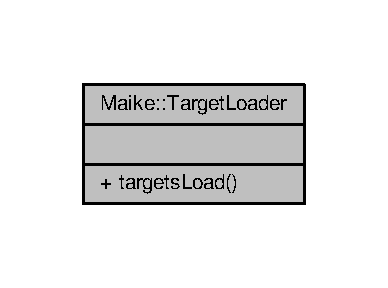
\includegraphics[width=186pt]{class_maike_1_1_target_loader__coll__graph}
\end{center}
\end{figure}
\subsection*{Public Member Functions}
\begin{DoxyCompactItemize}
\item 
virtual void \hyperlink{class_maike_1_1_target_loader_a65f95971ea6aba4913e8cb5b8b88bc71}{targets\+Load} (const char $\ast$name\+\_\+src, const char $\ast$in\+\_\+dir, \hyperlink{class_maike_1_1_spider}{Spider} \&spider, \hyperlink{class_maike_1_1_dependency_graph}{Dependency\+Graph} \&graph)=0
\end{DoxyCompactItemize}


\subsection{Member Function Documentation}
\index{Maike\+::\+Target\+Loader@{Maike\+::\+Target\+Loader}!targets\+Load@{targets\+Load}}
\index{targets\+Load@{targets\+Load}!Maike\+::\+Target\+Loader@{Maike\+::\+Target\+Loader}}
\subsubsection[{\texorpdfstring{targets\+Load(const char $\ast$name\+\_\+src, const char $\ast$in\+\_\+dir, Spider \&spider, Dependency\+Graph \&graph)=0}{targetsLoad(const char *name_src, const char *in_dir, Spider &spider, DependencyGraph &graph)=0}}]{\setlength{\rightskip}{0pt plus 5cm}virtual void Maike\+::\+Target\+Loader\+::targets\+Load (
\begin{DoxyParamCaption}
\item[{const char $\ast$}]{name\+\_\+src, }
\item[{const char $\ast$}]{in\+\_\+dir, }
\item[{{\bf Spider} \&}]{spider, }
\item[{{\bf Dependency\+Graph} \&}]{graph}
\end{DoxyParamCaption}
)\hspace{0.3cm}{\ttfamily [pure virtual]}}\hypertarget{class_maike_1_1_target_loader_a65f95971ea6aba4913e8cb5b8b88bc71}{}\label{class_maike_1_1_target_loader_a65f95971ea6aba4913e8cb5b8b88bc71}


The documentation for this class was generated from the following file\+:\begin{DoxyCompactItemize}
\item 
\hyperlink{targetloader_8hpp}{targetloader.\+hpp}\end{DoxyCompactItemize}

\hypertarget{class_maike_1_1_dependency_graph_1_1_target_processor}{}\section{Maike\+:\+:Dependency\+Graph\+:\+:Target\+Processor Class Reference}
\label{class_maike_1_1_dependency_graph_1_1_target_processor}\index{Maike\+::\+Dependency\+Graph\+::\+Target\+Processor@{Maike\+::\+Dependency\+Graph\+::\+Target\+Processor}}


{\ttfamily \#include $<$dependencygraph.\+hpp$>$}



Inheritance diagram for Maike\+:\+:Dependency\+Graph\+:\+:Target\+Processor\+:\nopagebreak
\begin{figure}[H]
\begin{center}
\leavevmode
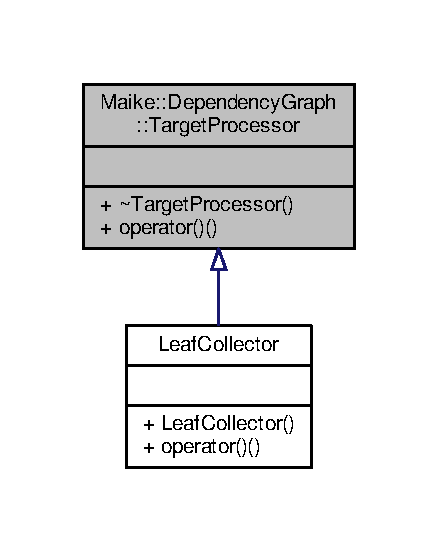
\includegraphics[width=210pt]{class_maike_1_1_dependency_graph_1_1_target_processor__inherit__graph}
\end{center}
\end{figure}


Collaboration diagram for Maike\+:\+:Dependency\+Graph\+:\+:Target\+Processor\+:\nopagebreak
\begin{figure}[H]
\begin{center}
\leavevmode
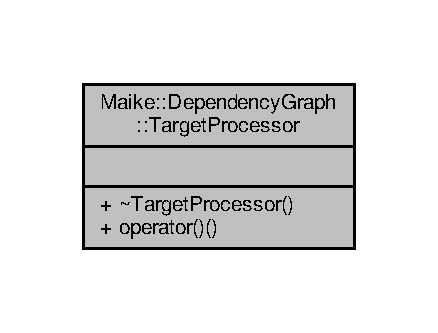
\includegraphics[width=210pt]{class_maike_1_1_dependency_graph_1_1_target_processor__coll__graph}
\end{center}
\end{figure}
\subsection*{Public Member Functions}
\begin{DoxyCompactItemize}
\item 
virtual \hyperlink{class_maike_1_1_dependency_graph_1_1_target_processor_ae7e9b15b40e33c74735681e29c5010a9}{$\sim$\+Target\+Processor} ()=default
\item 
virtual void \hyperlink{class_maike_1_1_dependency_graph_1_1_target_processor_af9bbe41827153c1bcbb01c62423a7850}{operator()} (\hyperlink{class_maike_1_1_dependency_graph}{Dependency\+Graph} \&graph, \hyperlink{class_maike_1_1_target}{Target} \&target)=0
\end{DoxyCompactItemize}


\subsection{Constructor \& Destructor Documentation}
\index{Maike\+::\+Dependency\+Graph\+::\+Target\+Processor@{Maike\+::\+Dependency\+Graph\+::\+Target\+Processor}!````~Target\+Processor@{$\sim$\+Target\+Processor}}
\index{````~Target\+Processor@{$\sim$\+Target\+Processor}!Maike\+::\+Dependency\+Graph\+::\+Target\+Processor@{Maike\+::\+Dependency\+Graph\+::\+Target\+Processor}}
\subsubsection[{\texorpdfstring{$\sim$\+Target\+Processor()=default}{~TargetProcessor()=default}}]{\setlength{\rightskip}{0pt plus 5cm}virtual Maike\+::\+Dependency\+Graph\+::\+Target\+Processor\+::$\sim$\+Target\+Processor (
\begin{DoxyParamCaption}
{}
\end{DoxyParamCaption}
)\hspace{0.3cm}{\ttfamily [virtual]}, {\ttfamily [default]}}\hypertarget{class_maike_1_1_dependency_graph_1_1_target_processor_ae7e9b15b40e33c74735681e29c5010a9}{}\label{class_maike_1_1_dependency_graph_1_1_target_processor_ae7e9b15b40e33c74735681e29c5010a9}


\subsection{Member Function Documentation}
\index{Maike\+::\+Dependency\+Graph\+::\+Target\+Processor@{Maike\+::\+Dependency\+Graph\+::\+Target\+Processor}!operator()@{operator()}}
\index{operator()@{operator()}!Maike\+::\+Dependency\+Graph\+::\+Target\+Processor@{Maike\+::\+Dependency\+Graph\+::\+Target\+Processor}}
\subsubsection[{\texorpdfstring{operator()(\+Dependency\+Graph \&graph, Target \&target)=0}{operator()(DependencyGraph &graph, Target &target)=0}}]{\setlength{\rightskip}{0pt plus 5cm}virtual void Maike\+::\+Dependency\+Graph\+::\+Target\+Processor\+::operator() (
\begin{DoxyParamCaption}
\item[{{\bf Dependency\+Graph} \&}]{graph, }
\item[{{\bf Target} \&}]{target}
\end{DoxyParamCaption}
)\hspace{0.3cm}{\ttfamily [pure virtual]}}\hypertarget{class_maike_1_1_dependency_graph_1_1_target_processor_af9bbe41827153c1bcbb01c62423a7850}{}\label{class_maike_1_1_dependency_graph_1_1_target_processor_af9bbe41827153c1bcbb01c62423a7850}


Implemented in \hyperlink{class_leaf_collector_ad6eefbdbcf3710390449fab9aa8dfbfb}{Leaf\+Collector}.



The documentation for this class was generated from the following file\+:\begin{DoxyCompactItemize}
\item 
\hyperlink{dependencygraph_8hpp}{dependencygraph.\+hpp}\end{DoxyCompactItemize}

\hypertarget{struct_maike_1_1_twins}{}\section{Maike\+:\+:Twins$<$ T $>$ Struct Template Reference}
\label{struct_maike_1_1_twins}\index{Maike\+::\+Twins$<$ T $>$@{Maike\+::\+Twins$<$ T $>$}}


{\ttfamily \#include $<$invoker.\+hpp$>$}



Inheritance diagram for Maike\+:\+:Twins$<$ T $>$\+:\nopagebreak
\begin{figure}[H]
\begin{center}
\leavevmode
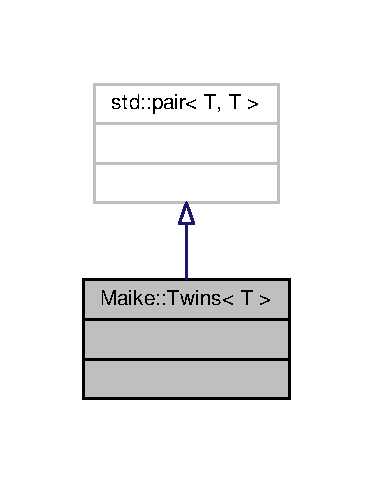
\includegraphics[width=179pt]{struct_maike_1_1_twins__inherit__graph}
\end{center}
\end{figure}


Collaboration diagram for Maike\+:\+:Twins$<$ T $>$\+:\nopagebreak
\begin{figure}[H]
\begin{center}
\leavevmode
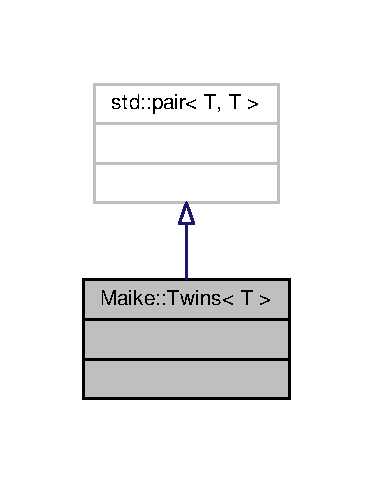
\includegraphics[width=179pt]{struct_maike_1_1_twins__coll__graph}
\end{center}
\end{figure}


The documentation for this struct was generated from the following file\+:\begin{DoxyCompactItemize}
\item 
\hyperlink{invoker_8hpp}{invoker.\+hpp}\end{DoxyCompactItemize}

\chapter{File Documentation}
\hypertarget{dependency_8cpp}{}\section{dependency.\+cpp File Reference}
\label{dependency_8cpp}\index{dependency.\+cpp@{dependency.\+cpp}}
{\ttfamily \#include \char`\"{}dependency.\+hpp\char`\"{}}\\*
Include dependency graph for dependency.\+cpp\+:\nopagebreak
\begin{figure}[H]
\begin{center}
\leavevmode
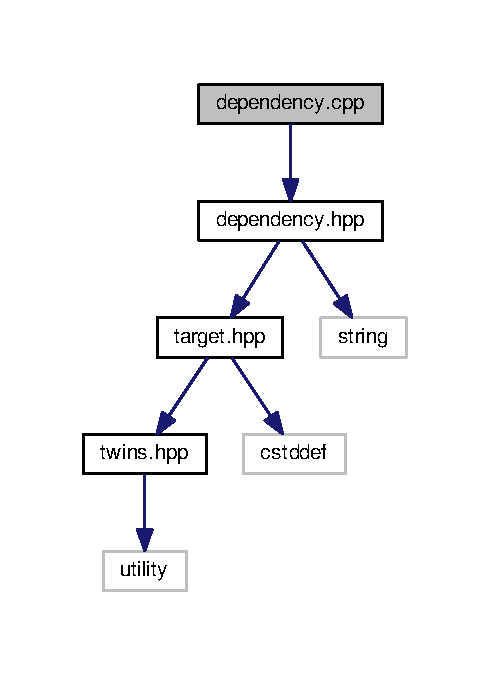
\includegraphics[width=235pt]{dependency_8cpp__incl}
\end{center}
\end{figure}

\hypertarget{dependency_8hpp}{}\section{dependency.\+hpp File Reference}
\label{dependency_8hpp}\index{dependency.\+hpp@{dependency.\+hpp}}
{\ttfamily \#include \char`\"{}target.\+hpp\char`\"{}}\\*
{\ttfamily \#include $<$string$>$}\\*
Include dependency graph for dependency.\+hpp\+:\nopagebreak
\begin{figure}[H]
\begin{center}
\leavevmode
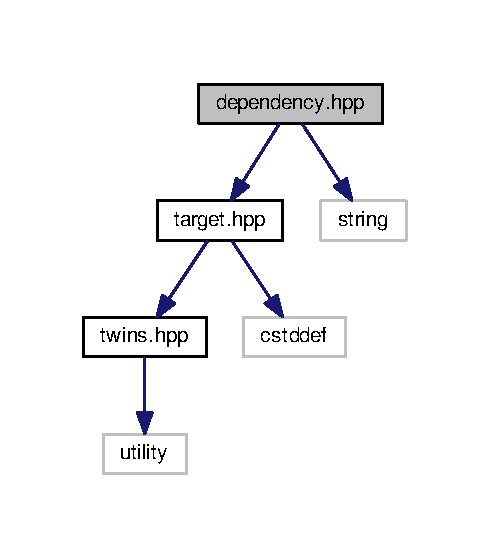
\includegraphics[width=235pt]{dependency_8hpp__incl}
\end{center}
\end{figure}
This graph shows which files directly or indirectly include this file\+:\nopagebreak
\begin{figure}[H]
\begin{center}
\leavevmode
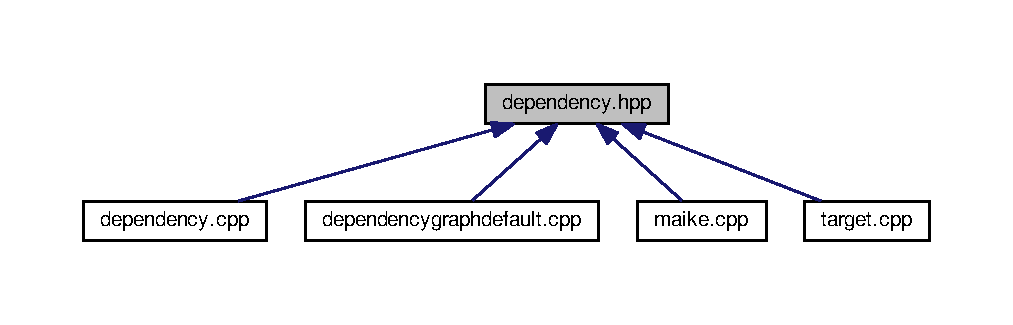
\includegraphics[width=350pt]{dependency_8hpp__dep__incl}
\end{center}
\end{figure}
\subsection*{Classes}
\begin{DoxyCompactItemize}
\item 
class \hyperlink{class_maike_1_1_dependency}{Maike\+::\+Dependency}
\end{DoxyCompactItemize}
\subsection*{Namespaces}
\begin{DoxyCompactItemize}
\item 
 \hyperlink{namespace_maike}{Maike}
\end{DoxyCompactItemize}

\hypertarget{dependencygraph_8hpp}{}\section{dependencygraph.\+hpp File Reference}
\label{dependencygraph_8hpp}\index{dependencygraph.\+hpp@{dependencygraph.\+hpp}}
{\ttfamily \#include $<$memory$>$}\\*
Include dependency graph for dependencygraph.\+hpp\+:\nopagebreak
\begin{figure}[H]
\begin{center}
\leavevmode
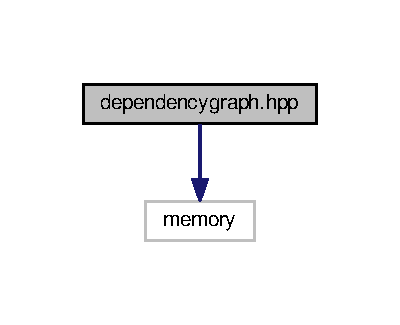
\includegraphics[width=192pt]{dependencygraph_8hpp__incl}
\end{center}
\end{figure}
This graph shows which files directly or indirectly include this file\+:\nopagebreak
\begin{figure}[H]
\begin{center}
\leavevmode
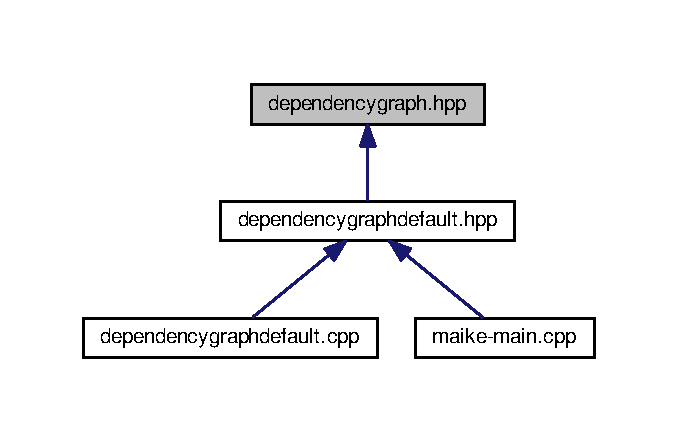
\includegraphics[width=326pt]{dependencygraph_8hpp__dep__incl}
\end{center}
\end{figure}
\subsection*{Classes}
\begin{DoxyCompactItemize}
\item 
class \hyperlink{class_maike_1_1_dependency_graph}{Maike\+::\+Dependency\+Graph}
\item 
class \hyperlink{class_maike_1_1_dependency_graph_1_1_target_processor}{Maike\+::\+Dependency\+Graph\+::\+Target\+Processor}
\end{DoxyCompactItemize}
\subsection*{Namespaces}
\begin{DoxyCompactItemize}
\item 
 \hyperlink{namespace_maike}{Maike}
\end{DoxyCompactItemize}

\hypertarget{dependencygraphdefault_8cpp}{}\section{dependencygraphdefault.\+cpp File Reference}
\label{dependencygraphdefault_8cpp}\index{dependencygraphdefault.\+cpp@{dependencygraphdefault.\+cpp}}
{\ttfamily \#include \char`\"{}dependencygraphdefault.\+hpp\char`\"{}}\\*
{\ttfamily \#include \char`\"{}target.\+hpp\char`\"{}}\\*
{\ttfamily \#include \char`\"{}dependency.\+hpp\char`\"{}}\\*
Include dependency graph for dependencygraphdefault.\+cpp\+:\nopagebreak
\begin{figure}[H]
\begin{center}
\leavevmode
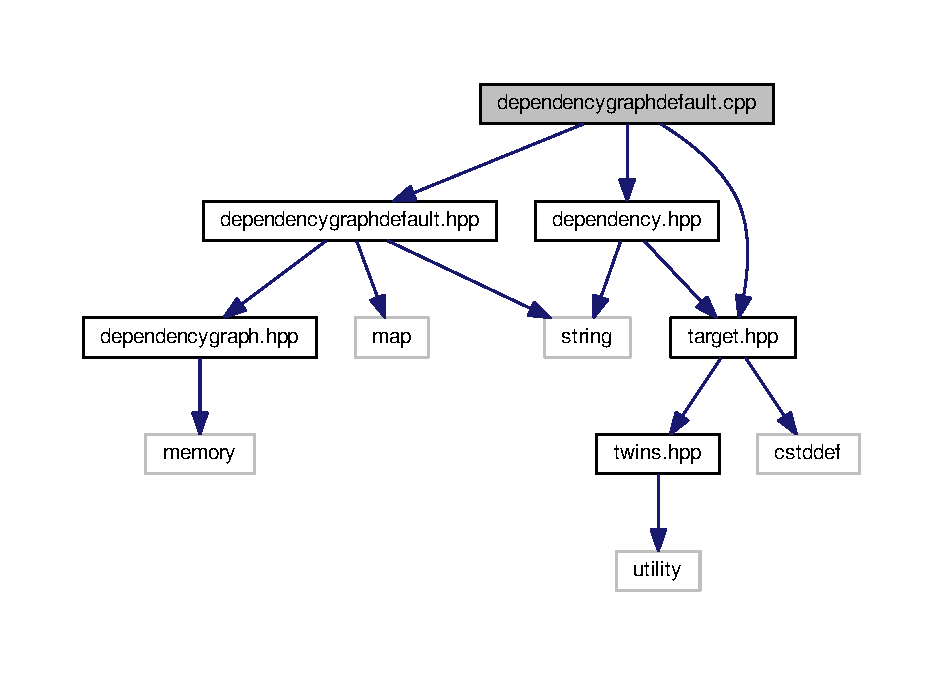
\includegraphics[width=350pt]{dependencygraphdefault_8cpp__incl}
\end{center}
\end{figure}

\hypertarget{dependencygraphdefault_8hpp}{}\section{dependencygraphdefault.\+hpp File Reference}
\label{dependencygraphdefault_8hpp}\index{dependencygraphdefault.\+hpp@{dependencygraphdefault.\+hpp}}
{\ttfamily \#include \char`\"{}dependencygraph.\+hpp\char`\"{}}\\*
{\ttfamily \#include $<$map$>$}\\*
{\ttfamily \#include $<$string$>$}\\*
Include dependency graph for dependencygraphdefault.\+hpp\+:\nopagebreak
\begin{figure}[H]
\begin{center}
\leavevmode
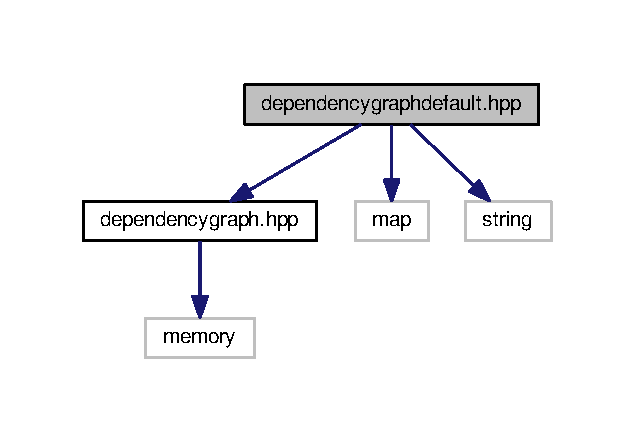
\includegraphics[width=305pt]{dependencygraphdefault_8hpp__incl}
\end{center}
\end{figure}
This graph shows which files directly or indirectly include this file\+:\nopagebreak
\begin{figure}[H]
\begin{center}
\leavevmode
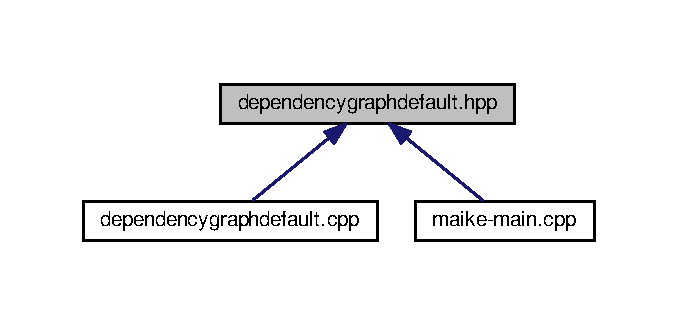
\includegraphics[width=326pt]{dependencygraphdefault_8hpp__dep__incl}
\end{center}
\end{figure}
\subsection*{Classes}
\begin{DoxyCompactItemize}
\item 
class \hyperlink{class_maike_1_1_dependency_graph_default}{Maike\+::\+Dependency\+Graph\+Default}
\end{DoxyCompactItemize}
\subsection*{Namespaces}
\begin{DoxyCompactItemize}
\item 
 \hyperlink{namespace_maike}{Maike}
\end{DoxyCompactItemize}

\hypertarget{invoker_8hpp}{}\section{invoker.\+hpp File Reference}
\label{invoker_8hpp}\index{invoker.\+hpp@{invoker.\+hpp}}
\subsection*{Classes}
\begin{DoxyCompactItemize}
\item 
struct \hyperlink{struct_maike_1_1_twins}{Maike\+::\+Twins$<$ T $>$}
\item 
class \hyperlink{class_maike_1_1_invoker}{Maike\+::\+Invoker}
\end{DoxyCompactItemize}
\subsection*{Namespaces}
\begin{DoxyCompactItemize}
\item 
 \hyperlink{namespace_maike}{Maike}
\end{DoxyCompactItemize}

\hypertarget{invokerreal_8hpp}{}\section{invokerreal.\+hpp File Reference}
\label{invokerreal_8hpp}\index{invokerreal.\+hpp@{invokerreal.\+hpp}}
{\ttfamily \#include \char`\"{}invokerreal.\+hpp\char`\"{}}\\*
Include dependency graph for invokerreal.\+hpp\+:\nopagebreak
\begin{figure}[H]
\begin{center}
\leavevmode
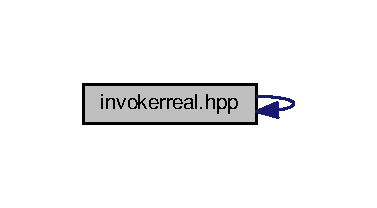
\includegraphics[width=181pt]{invokerreal_8hpp__incl}
\end{center}
\end{figure}
This graph shows which files directly or indirectly include this file\+:\nopagebreak
\begin{figure}[H]
\begin{center}
\leavevmode
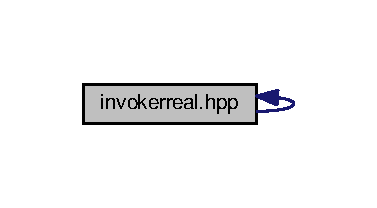
\includegraphics[width=181pt]{invokerreal_8hpp__dep__incl}
\end{center}
\end{figure}
\subsection*{Classes}
\begin{DoxyCompactItemize}
\item 
class \hyperlink{class_maike_1_1_invoker_real}{Maike\+::\+Invoker\+Real}
\end{DoxyCompactItemize}
\subsection*{Namespaces}
\begin{DoxyCompactItemize}
\item 
 \hyperlink{namespace_maike}{Maike}
\end{DoxyCompactItemize}

\hypertarget{maike-main_8cpp}{}\section{maike-\/main.cpp File Reference}
\label{maike-main_8cpp}\index{maike-\/main.\+cpp@{maike-\/main.\+cpp}}
{\ttfamily \#include \char`\"{}dependencygraphdefault.\+hpp\char`\"{}}\\*
{\ttfamily \#include \char`\"{}target.\+hpp\char`\"{}}\\*
{\ttfamily \#include $<$vector$>$}\\*
Include dependency graph for maike-\/main.cpp\+:\nopagebreak
\begin{figure}[H]
\begin{center}
\leavevmode
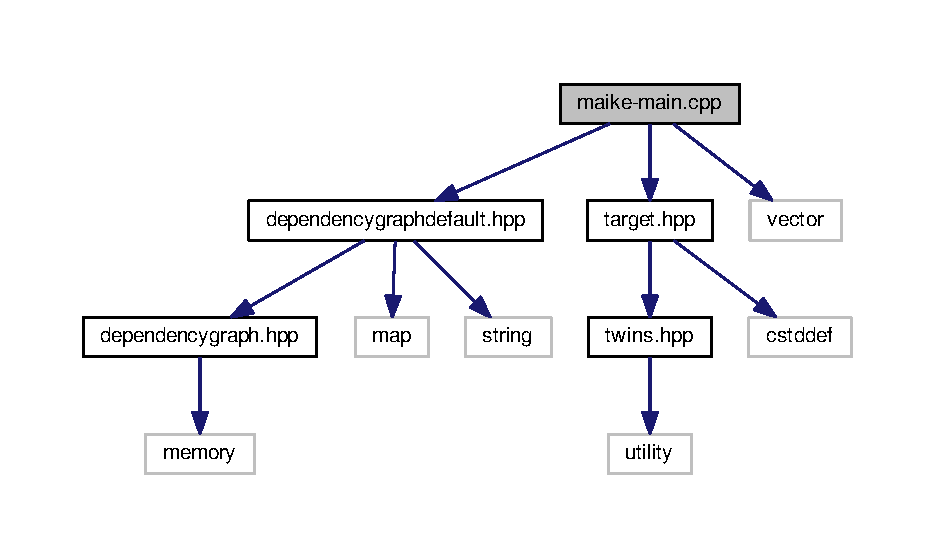
\includegraphics[width=350pt]{maike-main_8cpp__incl}
\end{center}
\end{figure}
\subsection*{Classes}
\begin{DoxyCompactItemize}
\item 
class \hyperlink{class_leaf_collector}{Leaf\+Collector}
\end{DoxyCompactItemize}
\subsection*{Functions}
\begin{DoxyCompactItemize}
\item 
int \hyperlink{maike-main_8cpp_a7a29781a20c5dd4153c3c1cecf0ff328}{main} (int argc, char $\ast$$\ast$args)
\end{DoxyCompactItemize}


\subsection{Function Documentation}
\index{maike-\/main.\+cpp@{maike-\/main.\+cpp}!main@{main}}
\index{main@{main}!maike-\/main.\+cpp@{maike-\/main.\+cpp}}
\subsubsection[{\texorpdfstring{main(int argc, char $\ast$$\ast$args)}{main(int argc, char **args)}}]{\setlength{\rightskip}{0pt plus 5cm}int main (
\begin{DoxyParamCaption}
\item[{int}]{argc, }
\item[{char $\ast$$\ast$}]{args}
\end{DoxyParamCaption}
)}\hypertarget{maike-main_8cpp_a7a29781a20c5dd4153c3c1cecf0ff328}{}\label{maike-main_8cpp_a7a29781a20c5dd4153c3c1cecf0ff328}

\hypertarget{maike_8cpp}{}\section{maike.\+cpp File Reference}
\label{maike_8cpp}\index{maike.\+cpp@{maike.\+cpp}}
{\ttfamily \#include \char`\"{}maike.\+hpp\char`\"{}}\\*
{\ttfamily \#include \char`\"{}target.\+hpp\char`\"{}}\\*
{\ttfamily \#include \char`\"{}dependency.\+hpp\char`\"{}}\\*
{\ttfamily \#include $<$vector$>$}\\*
{\ttfamily \#include $<$stack$>$}\\*
Include dependency graph for maike.\+cpp\+:\nopagebreak
\begin{figure}[H]
\begin{center}
\leavevmode
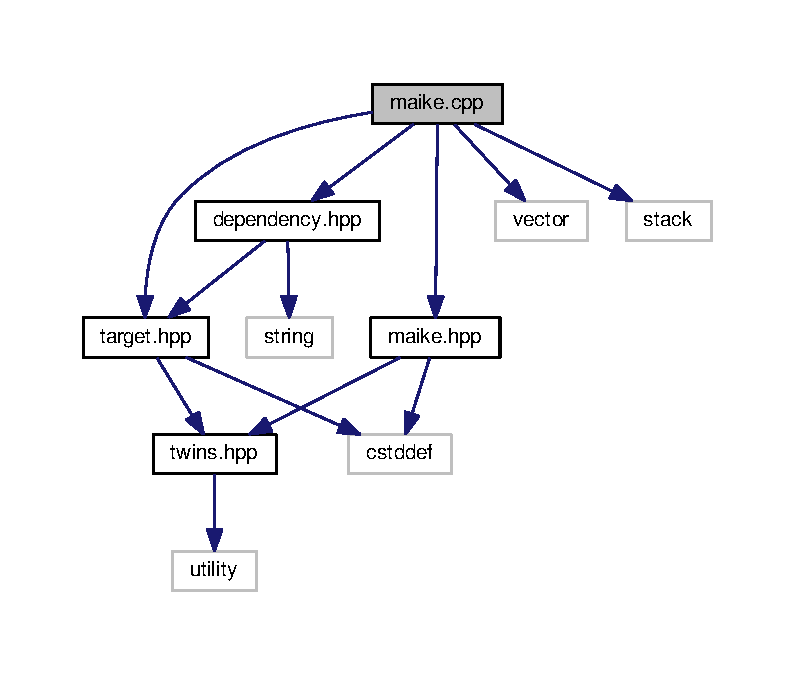
\includegraphics[width=350pt]{maike_8cpp__incl}
\end{center}
\end{figure}

\hypertarget{maike_8hpp}{}\section{maike.\+hpp File Reference}
\label{maike_8hpp}\index{maike.\+hpp@{maike.\+hpp}}
{\ttfamily \#include \char`\"{}twins.\+hpp\char`\"{}}\\*
{\ttfamily \#include $<$cstddef$>$}\\*
Include dependency graph for maike.\+hpp\+:\nopagebreak
\begin{figure}[H]
\begin{center}
\leavevmode
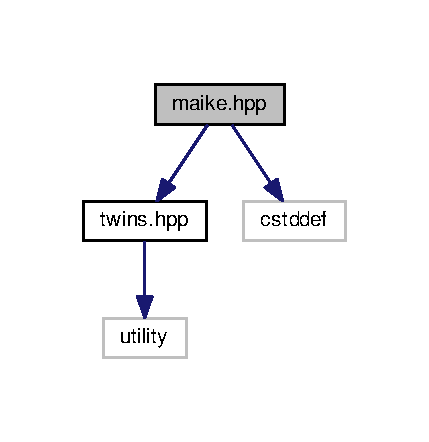
\includegraphics[width=206pt]{maike_8hpp__incl}
\end{center}
\end{figure}
This graph shows which files directly or indirectly include this file\+:\nopagebreak
\begin{figure}[H]
\begin{center}
\leavevmode
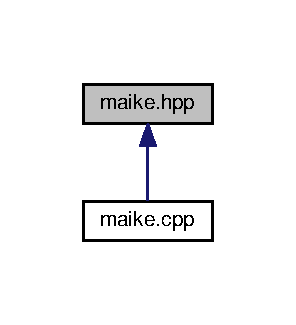
\includegraphics[width=142pt]{maike_8hpp__dep__incl}
\end{center}
\end{figure}
\subsection*{Namespaces}
\begin{DoxyCompactItemize}
\item 
 \hyperlink{namespace_maike}{Maike}
\end{DoxyCompactItemize}
\subsection*{Functions}
\begin{DoxyCompactItemize}
\item 
void \hyperlink{namespace_maike_a1b65c50ccc0ce45272d1eb6557057ec0}{Maike\+::build\+Branch} (\hyperlink{class_maike_1_1_target}{Target} \&target, \hyperlink{class_maike_1_1_invoker}{Invoker} \&invoker, size\+\_\+t targets\+\_\+count)
\item 
void \hyperlink{namespace_maike_aed76b0165d074646da9cfa1ad7bfc5b7}{Maike\+::build\+All} (\hyperlink{struct_maike_1_1_twins}{Twins}$<$ \hyperlink{class_maike_1_1_target}{Target} $\ast$ $>$ leafs, \hyperlink{class_maike_1_1_invoker}{Invoker} \&invoker, size\+\_\+t targets\+\_\+count)
\end{DoxyCompactItemize}

\hypertarget{spider_8hpp}{}\section{spider.\+hpp File Reference}
\label{spider_8hpp}\index{spider.\+hpp@{spider.\+hpp}}
{\ttfamily \#include $<$memory$>$}\\*
Include dependency graph for spider.\+hpp\+:\nopagebreak
\begin{figure}[H]
\begin{center}
\leavevmode
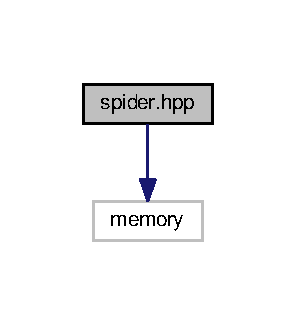
\includegraphics[width=142pt]{spider_8hpp__incl}
\end{center}
\end{figure}
\subsection*{Classes}
\begin{DoxyCompactItemize}
\item 
class \hyperlink{class_maike_1_1_spider}{Maike\+::\+Spider}
\end{DoxyCompactItemize}
\subsection*{Namespaces}
\begin{DoxyCompactItemize}
\item 
 \hyperlink{namespace_maike}{Maike}
\end{DoxyCompactItemize}

\hypertarget{target_8cpp}{}\section{target.\+cpp File Reference}
\label{target_8cpp}\index{target.\+cpp@{target.\+cpp}}
{\ttfamily \#include \char`\"{}target.\+hpp\char`\"{}}\\*
{\ttfamily \#include \char`\"{}dependency.\+hpp\char`\"{}}\\*
{\ttfamily \#include $<$vector$>$}\\*
Include dependency graph for target.\+cpp\+:\nopagebreak
\begin{figure}[H]
\begin{center}
\leavevmode
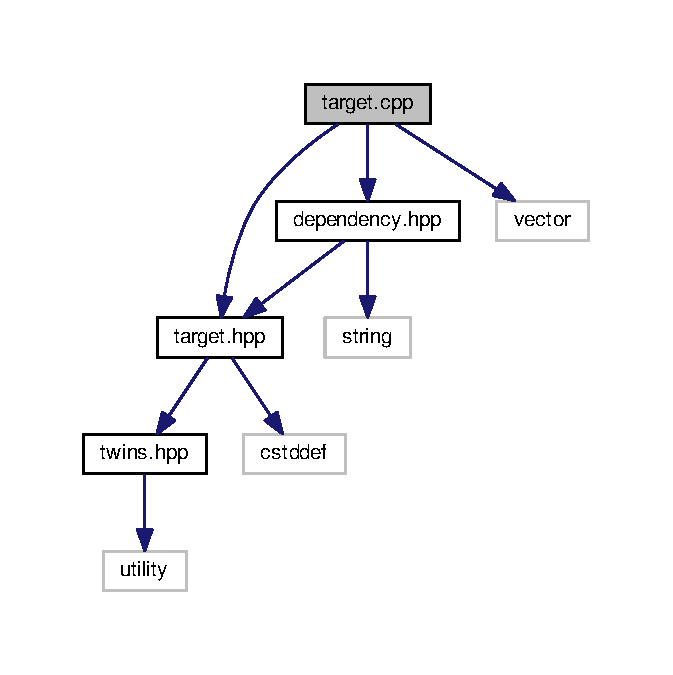
\includegraphics[width=323pt]{target_8cpp__incl}
\end{center}
\end{figure}

\hypertarget{target_8hpp}{}\section{target.\+hpp File Reference}
\label{target_8hpp}\index{target.\+hpp@{target.\+hpp}}
{\ttfamily \#include \char`\"{}twins.\+hpp\char`\"{}}\\*
{\ttfamily \#include $<$cstddef$>$}\\*
Include dependency graph for target.\+hpp\+:\nopagebreak
\begin{figure}[H]
\begin{center}
\leavevmode
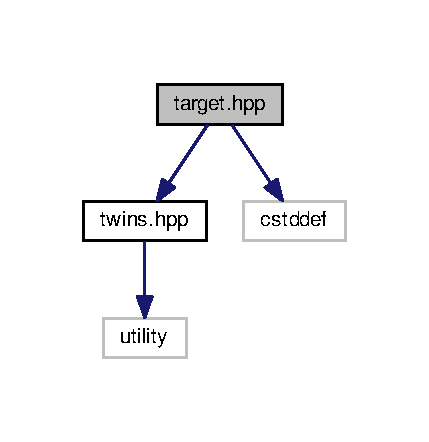
\includegraphics[width=206pt]{target_8hpp__incl}
\end{center}
\end{figure}
This graph shows which files directly or indirectly include this file\+:\nopagebreak
\begin{figure}[H]
\begin{center}
\leavevmode
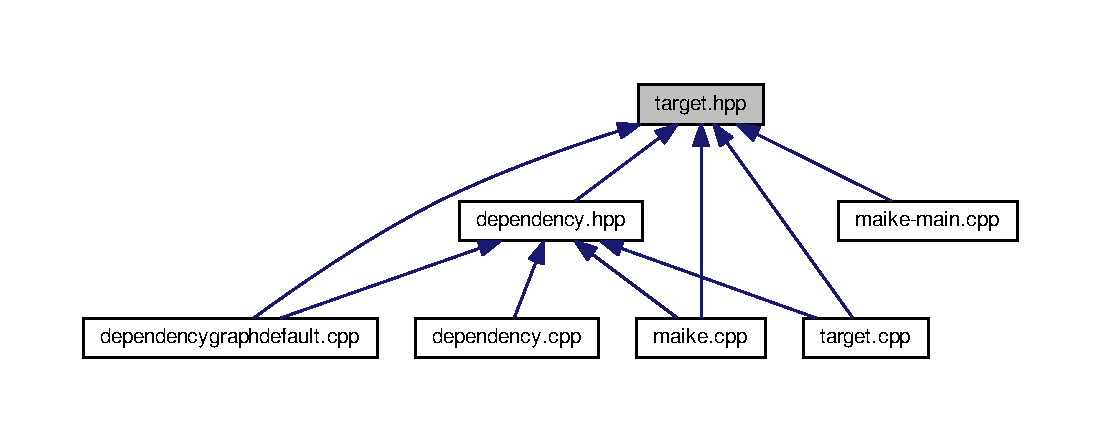
\includegraphics[width=350pt]{target_8hpp__dep__incl}
\end{center}
\end{figure}
\subsection*{Classes}
\begin{DoxyCompactItemize}
\item 
class \hyperlink{class_maike_1_1_target}{Maike\+::\+Target}
\end{DoxyCompactItemize}
\subsection*{Namespaces}
\begin{DoxyCompactItemize}
\item 
 \hyperlink{namespace_maike}{Maike}
\end{DoxyCompactItemize}

\hypertarget{targetloader_8hpp}{}\section{targetloader.\+hpp File Reference}
\label{targetloader_8hpp}\index{targetloader.\+hpp@{targetloader.\+hpp}}
\subsection*{Classes}
\begin{DoxyCompactItemize}
\item 
class \hyperlink{class_maike_1_1_target_loader}{Maike\+::\+Target\+Loader}
\end{DoxyCompactItemize}
\subsection*{Namespaces}
\begin{DoxyCompactItemize}
\item 
 \hyperlink{namespace_maike}{Maike}
\end{DoxyCompactItemize}

\hypertarget{twins_8hpp}{}\section{twins.\+hpp File Reference}
\label{twins_8hpp}\index{twins.\+hpp@{twins.\+hpp}}
{\ttfamily \#include $<$utility$>$}\\*
Include dependency graph for twins.\+hpp\+:\nopagebreak
\begin{figure}[H]
\begin{center}
\leavevmode
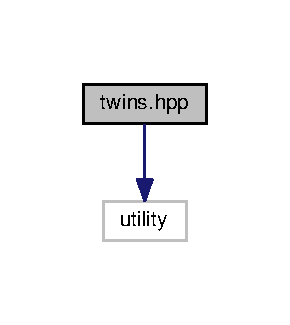
\includegraphics[width=139pt]{twins_8hpp__incl}
\end{center}
\end{figure}
This graph shows which files directly or indirectly include this file\+:\nopagebreak
\begin{figure}[H]
\begin{center}
\leavevmode
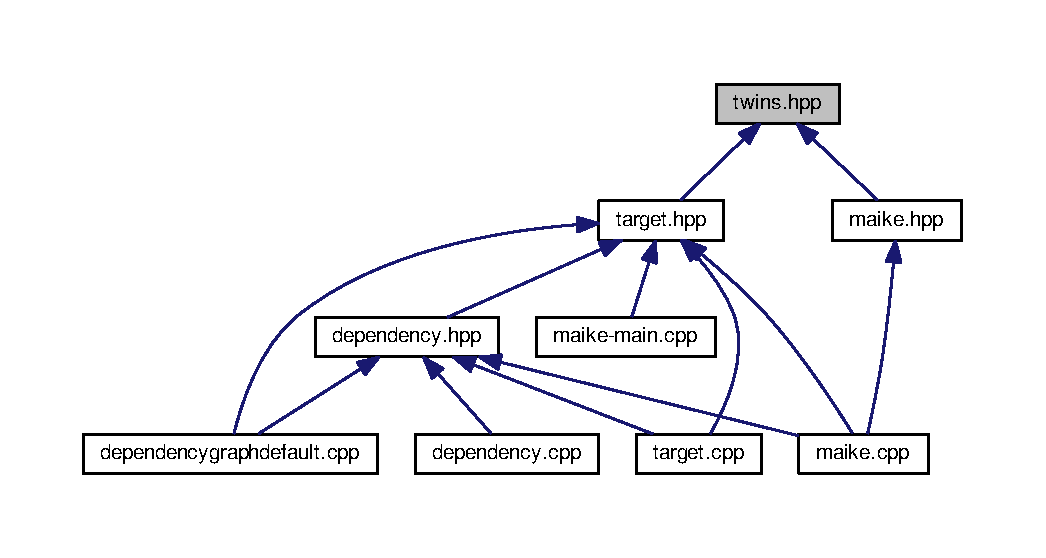
\includegraphics[width=350pt]{twins_8hpp__dep__incl}
\end{center}
\end{figure}
\subsection*{Classes}
\begin{DoxyCompactItemize}
\item 
struct \hyperlink{struct_maike_1_1_twins}{Maike\+::\+Twins$<$ T $>$}
\end{DoxyCompactItemize}
\subsection*{Namespaces}
\begin{DoxyCompactItemize}
\item 
 \hyperlink{namespace_maike}{Maike}
\end{DoxyCompactItemize}

%--- End generated contents ---

% Index
\backmatter
\newpage
\phantomsection
\clearemptydoublepage
\addcontentsline{toc}{chapter}{Index}
\printindex

\end{document}
